% Options for packages loaded elsewhere
\PassOptionsToPackage{unicode}{hyperref}
\PassOptionsToPackage{hyphens}{url}
%
\documentclass[
  12pt,
  a4paper,
  DIV=11,
  numbers=noendperiod]{scrreprt}

\usepackage{amsmath,amssymb}
\usepackage{setspace}
\usepackage{iftex}
\ifPDFTeX
  \usepackage[T1]{fontenc}
  \usepackage[utf8]{inputenc}
  \usepackage{textcomp} % provide euro and other symbols
\else % if luatex or xetex
  \usepackage{unicode-math}
  \defaultfontfeatures{Scale=MatchLowercase}
  \defaultfontfeatures[\rmfamily]{Ligatures=TeX,Scale=1}
\fi
\usepackage{lmodern}
\ifPDFTeX\else  
    % xetex/luatex font selection
\fi
% Use upquote if available, for straight quotes in verbatim environments
\IfFileExists{upquote.sty}{\usepackage{upquote}}{}
\IfFileExists{microtype.sty}{% use microtype if available
  \usepackage[]{microtype}
  \UseMicrotypeSet[protrusion]{basicmath} % disable protrusion for tt fonts
}{}
\usepackage{xcolor}
\setlength{\emergencystretch}{3em} % prevent overfull lines
\setcounter{secnumdepth}{5}
% Make \paragraph and \subparagraph free-standing
\ifx\paragraph\undefined\else
  \let\oldparagraph\paragraph
  \renewcommand{\paragraph}[1]{\oldparagraph{#1}\mbox{}}
\fi
\ifx\subparagraph\undefined\else
  \let\oldsubparagraph\subparagraph
  \renewcommand{\subparagraph}[1]{\oldsubparagraph{#1}\mbox{}}
\fi

\usepackage{color}
\usepackage{fancyvrb}
\newcommand{\VerbBar}{|}
\newcommand{\VERB}{\Verb[commandchars=\\\{\}]}
\DefineVerbatimEnvironment{Highlighting}{Verbatim}{commandchars=\\\{\}}
% Add ',fontsize=\small' for more characters per line
\usepackage{framed}
\definecolor{shadecolor}{RGB}{241,243,245}
\newenvironment{Shaded}{\begin{snugshade}}{\end{snugshade}}
\newcommand{\AlertTok}[1]{\textcolor[rgb]{0.68,0.00,0.00}{#1}}
\newcommand{\AnnotationTok}[1]{\textcolor[rgb]{0.37,0.37,0.37}{#1}}
\newcommand{\AttributeTok}[1]{\textcolor[rgb]{0.40,0.45,0.13}{#1}}
\newcommand{\BaseNTok}[1]{\textcolor[rgb]{0.68,0.00,0.00}{#1}}
\newcommand{\BuiltInTok}[1]{\textcolor[rgb]{0.00,0.23,0.31}{#1}}
\newcommand{\CharTok}[1]{\textcolor[rgb]{0.13,0.47,0.30}{#1}}
\newcommand{\CommentTok}[1]{\textcolor[rgb]{0.37,0.37,0.37}{#1}}
\newcommand{\CommentVarTok}[1]{\textcolor[rgb]{0.37,0.37,0.37}{\textit{#1}}}
\newcommand{\ConstantTok}[1]{\textcolor[rgb]{0.56,0.35,0.01}{#1}}
\newcommand{\ControlFlowTok}[1]{\textcolor[rgb]{0.00,0.23,0.31}{#1}}
\newcommand{\DataTypeTok}[1]{\textcolor[rgb]{0.68,0.00,0.00}{#1}}
\newcommand{\DecValTok}[1]{\textcolor[rgb]{0.68,0.00,0.00}{#1}}
\newcommand{\DocumentationTok}[1]{\textcolor[rgb]{0.37,0.37,0.37}{\textit{#1}}}
\newcommand{\ErrorTok}[1]{\textcolor[rgb]{0.68,0.00,0.00}{#1}}
\newcommand{\ExtensionTok}[1]{\textcolor[rgb]{0.00,0.23,0.31}{#1}}
\newcommand{\FloatTok}[1]{\textcolor[rgb]{0.68,0.00,0.00}{#1}}
\newcommand{\FunctionTok}[1]{\textcolor[rgb]{0.28,0.35,0.67}{#1}}
\newcommand{\ImportTok}[1]{\textcolor[rgb]{0.00,0.46,0.62}{#1}}
\newcommand{\InformationTok}[1]{\textcolor[rgb]{0.37,0.37,0.37}{#1}}
\newcommand{\KeywordTok}[1]{\textcolor[rgb]{0.00,0.23,0.31}{#1}}
\newcommand{\NormalTok}[1]{\textcolor[rgb]{0.00,0.23,0.31}{#1}}
\newcommand{\OperatorTok}[1]{\textcolor[rgb]{0.37,0.37,0.37}{#1}}
\newcommand{\OtherTok}[1]{\textcolor[rgb]{0.00,0.23,0.31}{#1}}
\newcommand{\PreprocessorTok}[1]{\textcolor[rgb]{0.68,0.00,0.00}{#1}}
\newcommand{\RegionMarkerTok}[1]{\textcolor[rgb]{0.00,0.23,0.31}{#1}}
\newcommand{\SpecialCharTok}[1]{\textcolor[rgb]{0.37,0.37,0.37}{#1}}
\newcommand{\SpecialStringTok}[1]{\textcolor[rgb]{0.13,0.47,0.30}{#1}}
\newcommand{\StringTok}[1]{\textcolor[rgb]{0.13,0.47,0.30}{#1}}
\newcommand{\VariableTok}[1]{\textcolor[rgb]{0.07,0.07,0.07}{#1}}
\newcommand{\VerbatimStringTok}[1]{\textcolor[rgb]{0.13,0.47,0.30}{#1}}
\newcommand{\WarningTok}[1]{\textcolor[rgb]{0.37,0.37,0.37}{\textit{#1}}}

\providecommand{\tightlist}{%
  \setlength{\itemsep}{0pt}\setlength{\parskip}{0pt}}\usepackage{longtable,booktabs,array}
\usepackage{calc} % for calculating minipage widths
% Correct order of tables after \paragraph or \subparagraph
\usepackage{etoolbox}
\makeatletter
\patchcmd\longtable{\par}{\if@noskipsec\mbox{}\fi\par}{}{}
\makeatother
% Allow footnotes in longtable head/foot
\IfFileExists{footnotehyper.sty}{\usepackage{footnotehyper}}{\usepackage{footnote}}
\makesavenoteenv{longtable}
\usepackage{graphicx}
\makeatletter
\def\maxwidth{\ifdim\Gin@nat@width>\linewidth\linewidth\else\Gin@nat@width\fi}
\def\maxheight{\ifdim\Gin@nat@height>\textheight\textheight\else\Gin@nat@height\fi}
\makeatother
% Scale images if necessary, so that they will not overflow the page
% margins by default, and it is still possible to overwrite the defaults
% using explicit options in \includegraphics[width, height, ...]{}
\setkeys{Gin}{width=\maxwidth,height=\maxheight,keepaspectratio}
% Set default figure placement to htbp
\makeatletter
\def\fps@figure{htbp}
\makeatother

\usepackage{indentfirst}
\usepackage{float}
\floatplacement{figure}{H}
\IfFileExists{plex-otf.sty}{
  %% Full TeXlive
  \usepackage[
    % math,
    RM={Scale=0.94},SS={Scale=0.94},SScon={Scale=0.94},TT={Scale=MatchLowercase,FakeStretch=0.9},
    DefaultFeatures={Ligatures=Common}
  ]{plex-otf}
  % \usepackage[Scale=MatchUppercase]{juliamono}
}{
  %% TinyTeX
  \usepackage{libertine}
}
\KOMAoption{captions}{tableheading}
\makeatletter
\@ifpackageloaded{caption}{}{\usepackage{caption}}
\AtBeginDocument{%
\ifdefined\contentsname
  \renewcommand*\contentsname{Содержание}
\else
  \newcommand\contentsname{Содержание}
\fi
\ifdefined\listfigurename
  \renewcommand*\listfigurename{Список иллюстраций}
\else
  \newcommand\listfigurename{Список иллюстраций}
\fi
\ifdefined\listtablename
  \renewcommand*\listtablename{Список таблиц}
\else
  \newcommand\listtablename{Список таблиц}
\fi
\ifdefined\figurename
  \renewcommand*\figurename{Рисунок}
\else
  \newcommand\figurename{Рисунок}
\fi
\ifdefined\tablename
  \renewcommand*\tablename{Таблица}
\else
  \newcommand\tablename{Таблица}
\fi
}
\@ifpackageloaded{float}{}{\usepackage{float}}
\floatstyle{ruled}
\@ifundefined{c@chapter}{\newfloat{codelisting}{h}{lop}}{\newfloat{codelisting}{h}{lop}[chapter]}
\floatname{codelisting}{Список}
\newcommand*\listoflistings{\listof{codelisting}{Листинги}}
\makeatother
\makeatletter
\makeatother
\makeatletter
\@ifpackageloaded{caption}{}{\usepackage{caption}}
\@ifpackageloaded{subcaption}{}{\usepackage{subcaption}}
\makeatother
\ifLuaTeX
\usepackage[bidi=basic]{babel}
\else
\usepackage[bidi=default]{babel}
\fi
\babelprovide[main,import]{russian}
\babelprovide[import]{english}
% get rid of language-specific shorthands (see #6817):
\let\LanguageShortHands\languageshorthands
\def\languageshorthands#1{}
\ifLuaTeX
  \usepackage{selnolig}  % disable illegal ligatures
\fi
\usepackage[style=gost-numeric,backend=biber,langhook=extras,autolang=other*]{biblatex}
\addbibresource{bib/cite.bib}
\usepackage{csquotes}
\usepackage{bookmark}

\IfFileExists{xurl.sty}{\usepackage{xurl}}{} % add URL line breaks if available
\urlstyle{same} % disable monospaced font for URLs
\hypersetup{
  pdftitle={Отчёта по лабораторной работе 3},
  pdfauthor={Нджову Нелиа},
  pdflang={ru-RU},
  hidelinks,
  pdfcreator={LaTeX via pandoc}}

\title{Отчёта по лабораторной работе 3}
\usepackage{etoolbox}
\makeatletter
\providecommand{\subtitle}[1]{% add subtitle to \maketitle
  \apptocmd{\@title}{\par {\large #1 \par}}{}{}
}
\makeatother
\subtitle{Иммитационное моделирование}
\author{Нджову Нелиа}
\date{}

\begin{document}
\maketitle

\renewcommand*\contentsname{Содержание}
{
\setcounter{tocdepth}{1}
\tableofcontents
}
\listoffigures
\listoftables
\setstretch{1.5}
\chapter{Цель
работы}\label{ux446ux435ux43bux44c-ux440ux430ux431ux43eux442ux44b}

Цель этой лабораторной работы использовать агентную модель для
моделирования daisyworld.

\chapter{Задание}\label{ux437ux430ux434ux430ux43dux438ux435}

\begin{enumerate}
\def\labelenumi{\arabic{enumi}.}
\item
  Реализация на Agents.jl
\item
  Базовая визуализация
\item
  Анимация модели
\item
  Динамика числа маргариток
\item
  Динамика модели
\item
  Базовая визуализация(параметры)
\item
  Динамика числа маргариток(параметы)
\item
  Динамика модели(параметры)
\end{enumerate}

\chapter{Теоретическое
введение}\label{ux442ux435ux43eux440ux435ux442ux438ux447ux435ux441ux43aux43eux435-ux432ux432ux435ux434ux435ux43dux438ux435}

\section{Агентный
подход}\label{ux430ux433ux435ux43dux442ux43dux44bux439-ux43fux43eux434ux445ux43eux434}

Агентный подход к имитационному моделированию (Agent-Based Modeling,
ABM) --- это метод исследования сложных систем, в котором поведение
системы возникает из взаимодействия множества автономных сущностей,
называемых агентами. Вместо того чтобы описывать систему глобальными
уравнениями, мы моделируем каждую индивидуальную единицу и правила её
поведения, а затем наблюдаем, какие коллективные паттерны появляются
снизу вверх. Этот подход особенно полезен, когда поведение системы
трудно предсказать из-за нелинейностей, гетерогенности участников или
адаптивных стратегий.

Любая агентная модель включает три основных элемента:

\begin{enumerate}
\def\labelenumi{\arabic{enumi}.}
\item
  Агенты --- это активные сущности. Они обладают свойствами, правилами
  поведения, целями и способностью к обучению или одаптации
\item
  Среда --- это пространство, в котором существуют агенты. Она может
  быть дискретной, непрерывной, сетевой и абстрактной. Среда также может
  иметь свои свойства (температура, ресурсы) и динамику (диффузия,
  обновление).
\item
  Взаимодействия --- правила, определяющие, как агенты влияют друг на
  друга и на среду. Они могут быть локальными, глобальными и через
  среду.
\end{enumerate}

Основные принципы агентного моделирования включает эмерджентность,
автономия, генерогенность и локальность

Преимущества агентного подхода включает гибкость, учёт индивидуальных
реализаций, адаптивность, наглядность и исследование

Этапы построения агентной модели: концептуализация, спецификация,
реализация, верификация, валидация, анализ и интерпретация

\section{Модель
Daisyworld}\label{ux43cux43eux434ux435ux43bux44c-daisyworld}

\textbf{Модель Daisyworld}, предложенная Джеймсом Лавлоком и Эндрю
Уотсоном (1983), иллюстрирует гипотезу Геи --- способность жизни
регулировать планетарные условия.

\subsection{Основные элементы
модели:}\label{ux43eux441ux43dux43eux432ux43dux44bux435-ux44dux43bux435ux43cux435ux43dux442ux44b-ux43cux43eux434ux435ux43bux438}

\textbf{1. Агенты (маргаритки)} - Два типа: \textbf{чёрные} (низкое
альбедо 0.25) и \textbf{белые} (высокое альбедо 0.75) - Свойства: тип,
возраст, альбедо, позиция на сетке - Правила: стареют, умирают при
достижении max\_age, размножаются в пустые соседние клетки

\textbf{2. Среда (планета)} - Дискретная сетка 30×30 клеток - Свойства:
температура каждой клетки, солнечная светимость - Динамика: диффузия
тепла между соседними клетками

\textbf{3. Взаимодействия} - Маргаритки \textbf{влияют на среду}: чёрные
поглощают тепло (нагревают), белые отражают тепло (охлаждают) - Среда
\textbf{влияет на агентов}: размножение возможно только при оптимальной
температуре (\textasciitilde22.5°C)

\subsection{Механизм
саморегуляции:}\label{ux43cux435ux445ux430ux43dux438ux437ux43c-ux441ux430ux43cux43eux440ux435ux433ux443ux43bux44fux446ux438ux438}

\begin{itemize}
\item
  \textbf{Слишком холодно} Чёрные маргаритки получают преимущество →
  распространяются → поглощают больше тепла → \textbf{планета
  нагревается}
\item
  \textbf{Слишком жарко} Белые маргаритки получают преимущество →
  распространяются → отражают больше тепла → \textbf{планета
  охлаждается} \textbar{}
\end{itemize}

\subsection{Ключевые
параметры:}\label{ux43aux43bux44eux447ux435ux432ux44bux435-ux43fux430ux440ux430ux43cux435ux442ux440ux44b}

\begin{longtable}[]{@{}ll@{}}
\toprule\noalign{}
Параметр & Значение \\
\midrule\noalign{}
\endhead
\bottomrule\noalign{}
\endlastfoot
Максимальный возраст & 25-40 шагов \\
Альбедо чёрных & 0.25 \\
Альбедо белых & 0.75 \\
Альбедо почвы & 0.4 \\
Оптимальная температура & 22.5°C \\
\end{longtable}

\subsection{Эмерджентное
поведение:}\label{ux44dux43cux435ux440ux434ux436ux435ux43dux442ux43dux43eux435-ux43fux43eux432ux435ux434ux435ux43dux438ux435}

Несмотря на простые локальные правила, глобально система демонстрирует
\textbf{поддержание стабильной температуры} в широком диапазоне
солнечной активности --- яркий пример саморегуляции без
централизованного управления.

\chapter{Выполнение лабораторной
работы}\label{ux432ux44bux43fux43eux43bux43dux435ux43dux438ux435-ux43bux430ux431ux43eux440ux430ux442ux43eux440ux43dux43eux439-ux440ux430ux431ux43eux442ux44b}

\section{1. Реализация на
Agents.jl}\label{ux440ux435ux430ux43bux438ux437ux430ux446ux438ux44f-ux43dux430-agents.jl}

Я создала файл src/daisyworld.jl и скопировала скрипт код, который мне
дали и запускала его. Этот скрипт код содержит ключевые функции
например, функции обновления температуры, функция рассеивания тепла,
функция воспроизведения ромашки, функция шага модели, функция солнечной
активности и т.д.(рис.~\ref{fig-001})

\begin{figure}

\centering{


\includegraphics[width=0.7\textwidth,height=\textheight]{image/pic1.png}

}

\caption{\label{fig-001}Ключевые функции модель Daisyworld}

\end{figure}%

\section{2. Базовая
визуализация}\label{ux431ux430ux437ux43eux432ux430ux44f-ux432ux438ux437ux443ux430ux43bux438ux437ux430ux446ux438ux44f}

Я создала файл scripts/daisyworld.jl и скопировала скрипт код, который
мне дали и запускала его. Это скрипт визуализации, который создает
моментальные снимки моделирования Daisyworld на разных временных
этапах(рис.~\ref{fig-002})

\begin{figure}

\centering{


\includegraphics[width=0.7\textwidth,height=\textheight]{image/pic5.png}

}

\caption{\label{fig-002}запуск код}

\end{figure}%

На полученных графиках видно, что в исходном состоянии ромашки
распределены случайным образом, но температура относительно
равномерная(рис.~\ref{fig-003})

\begin{figure}

\centering{

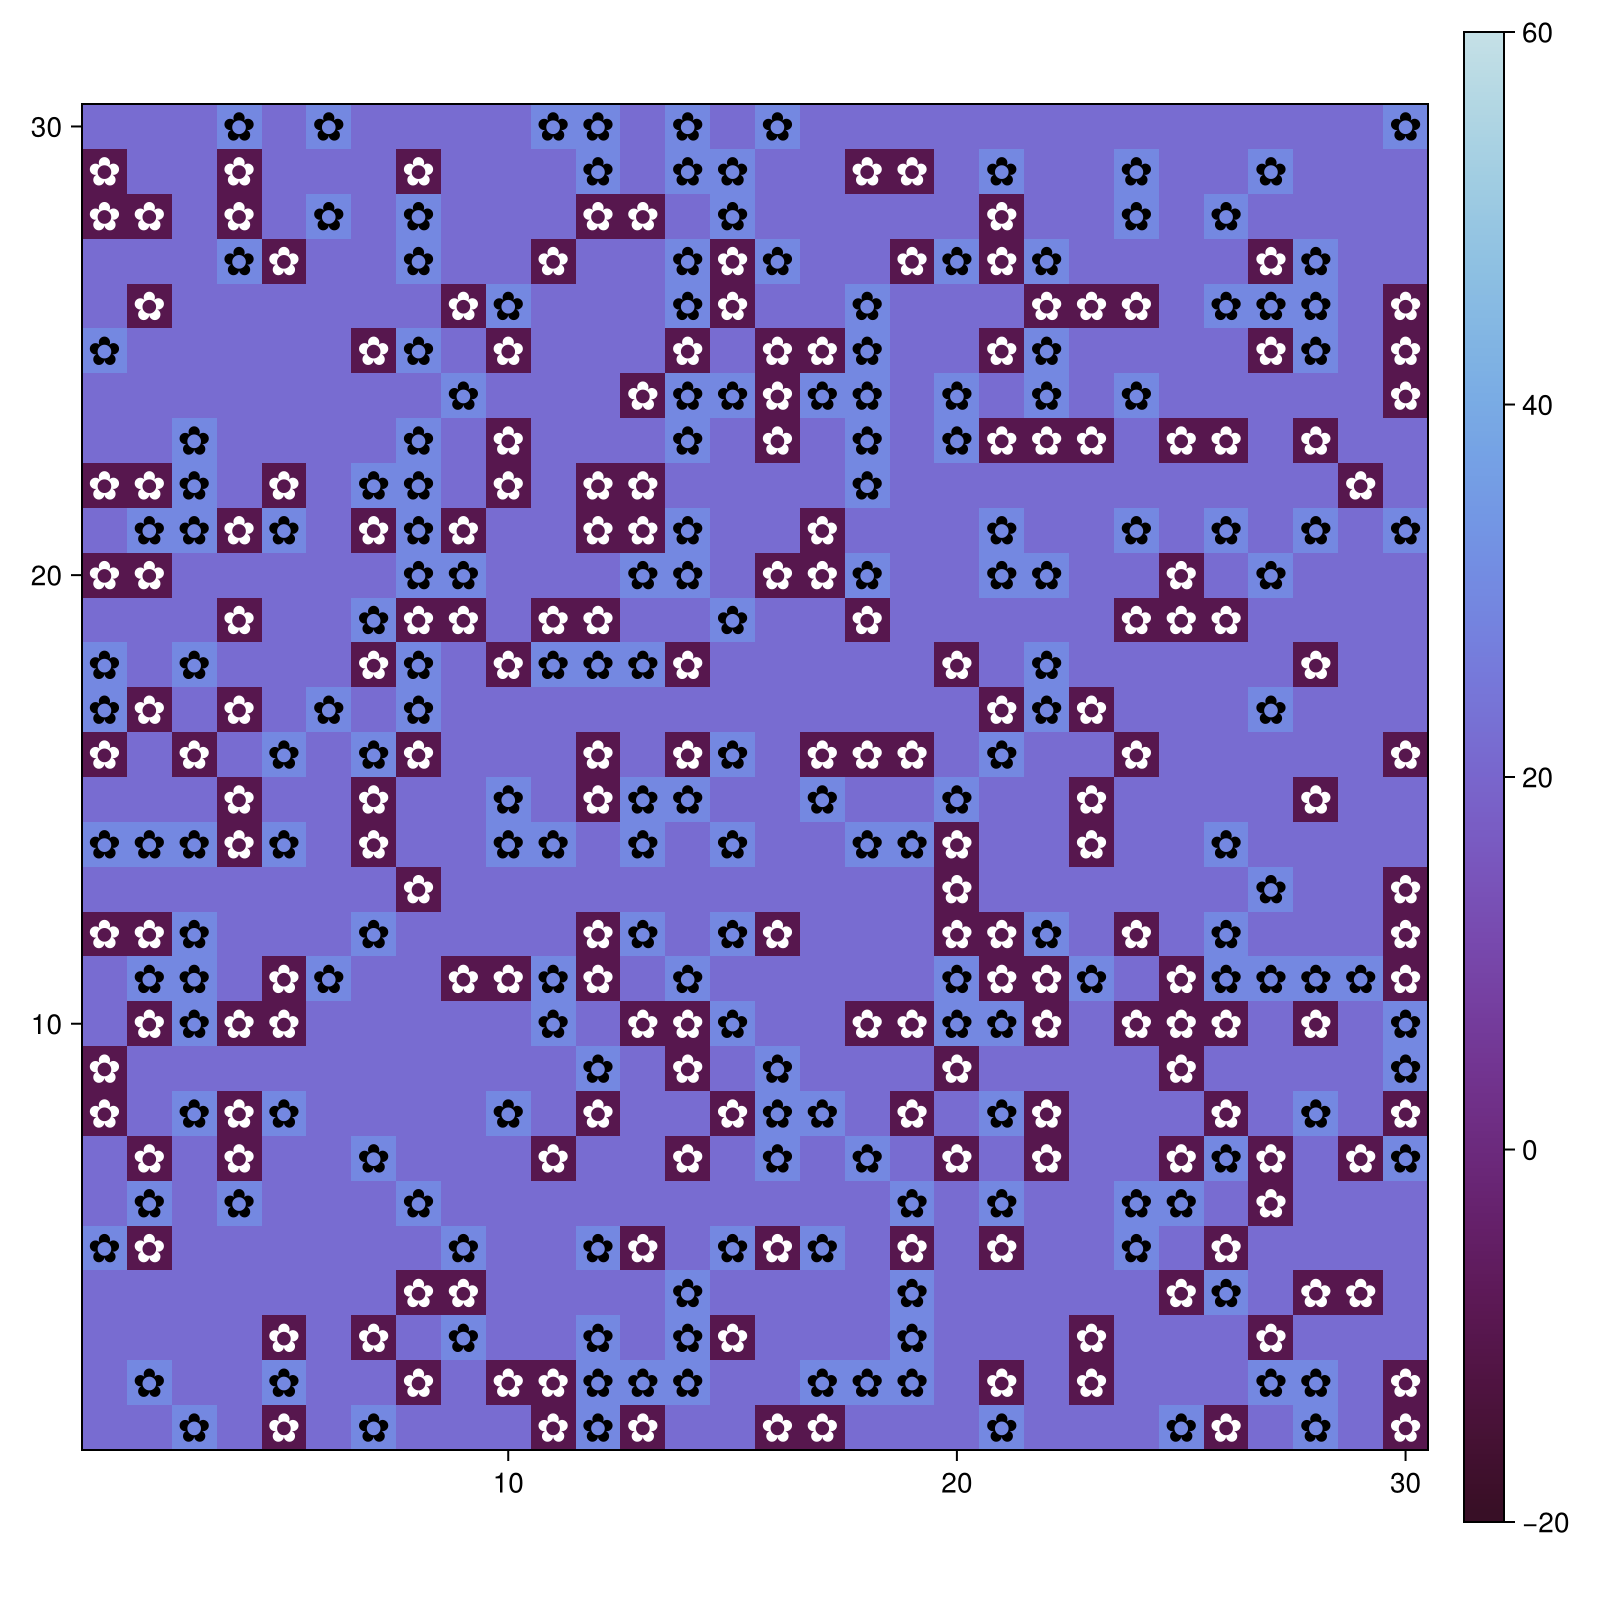
\includegraphics[width=0.7\textwidth,height=\textheight]{image/pic001.png}

}

\caption{\label{fig-003}Daisy\_step1}

\end{figure}%

После 5 шагов начинают формироваться локальные зоны нагрева (где
преобладают черные ромашки) и зоны охлаждения (где преобладают
белые)(\textbf{?@fig-004})
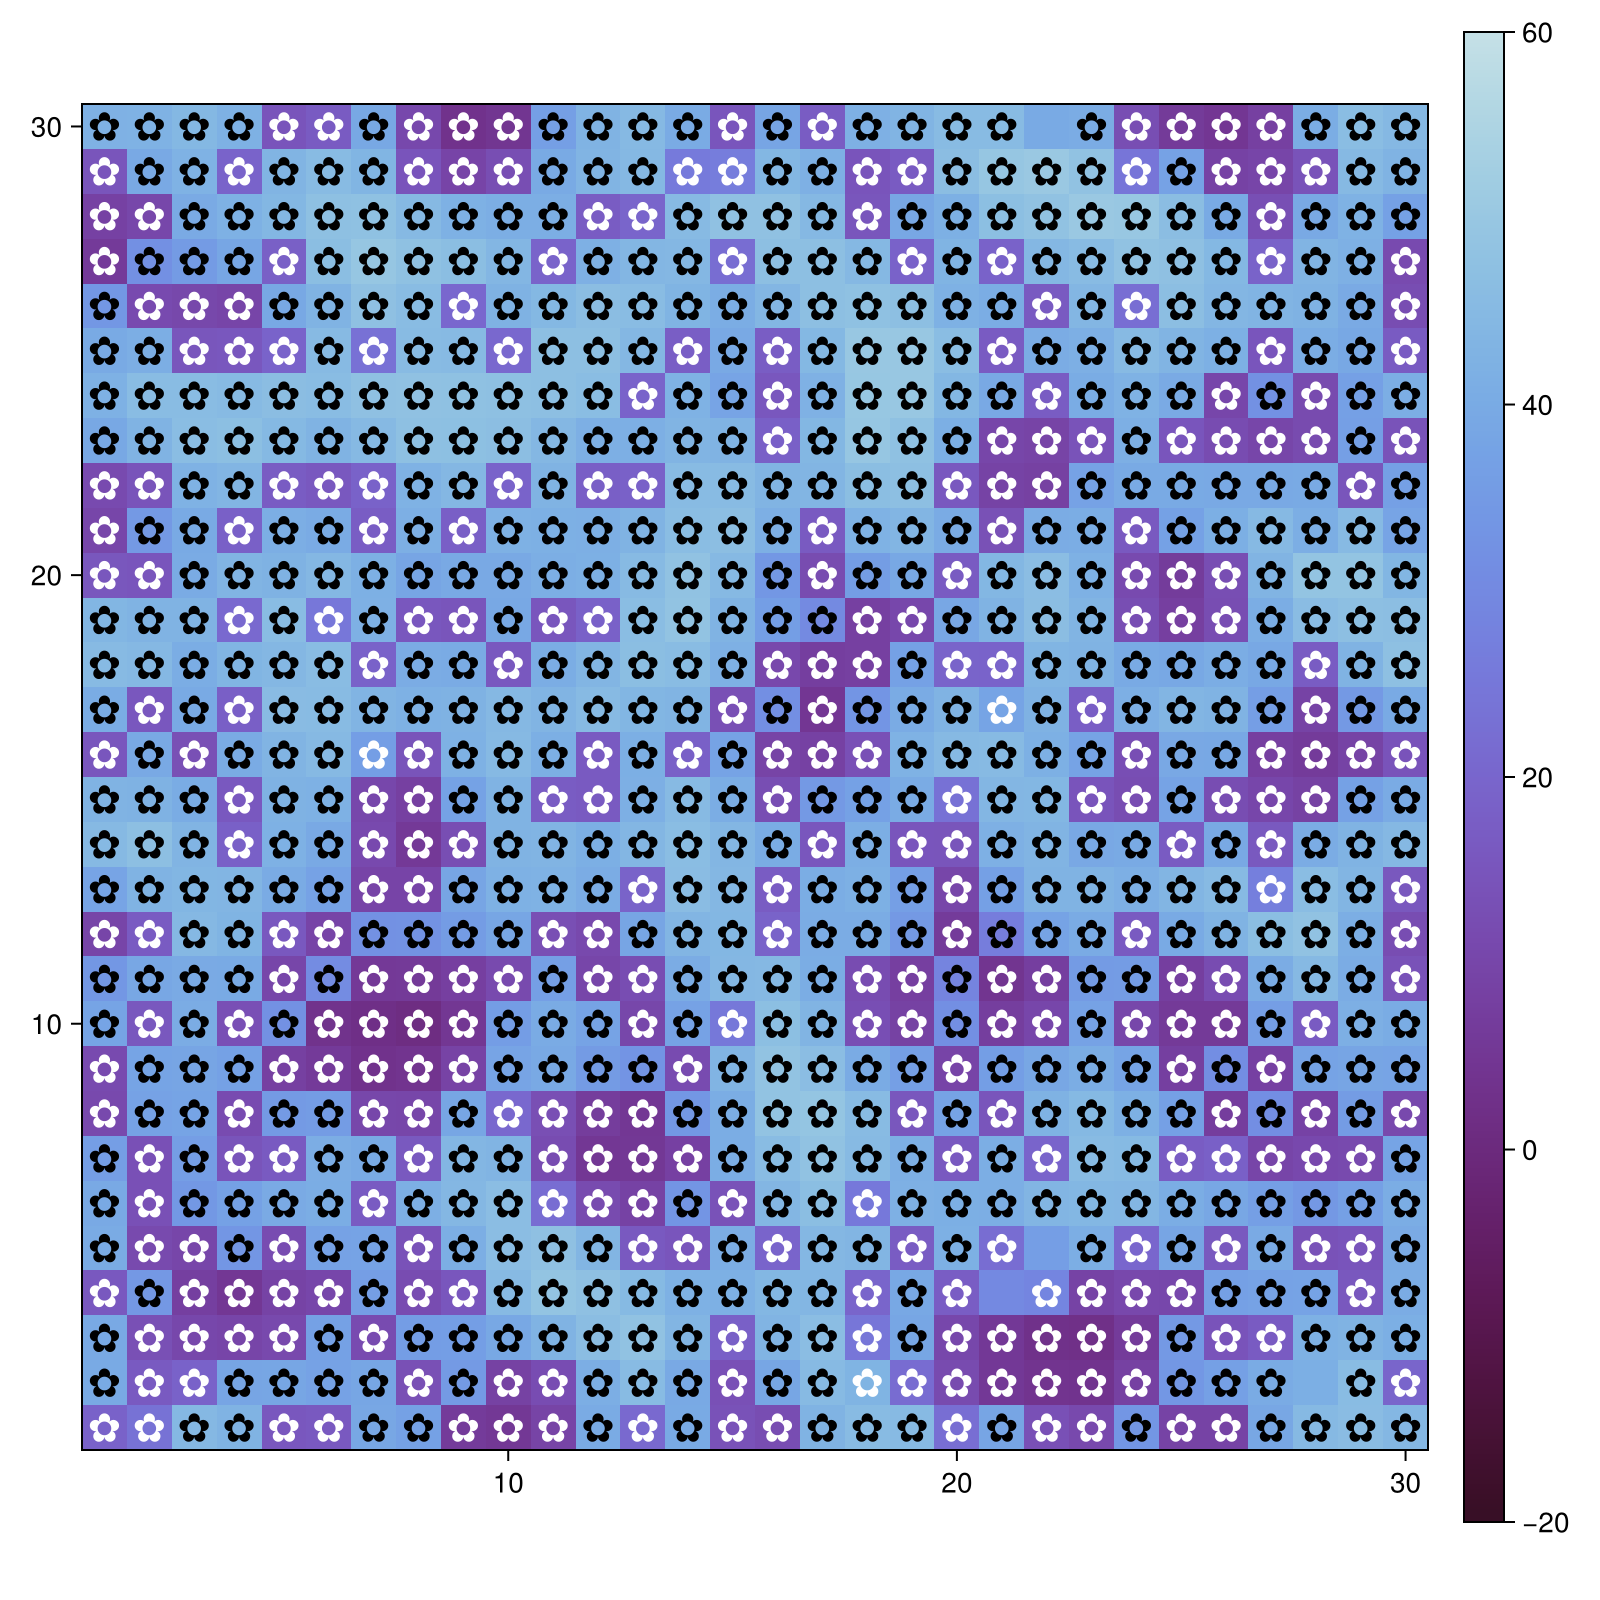
\includegraphics[width=0.7\textwidth,height=\textheight]{image/pic005.png}

После 40 шагов система достигает точки динамического равновесия.
Чередование черных и белых ромашек поддерживает глобальную температуру в
благоприятном диапазоне(рис.~\ref{fig-005})

\begin{figure}

\centering{

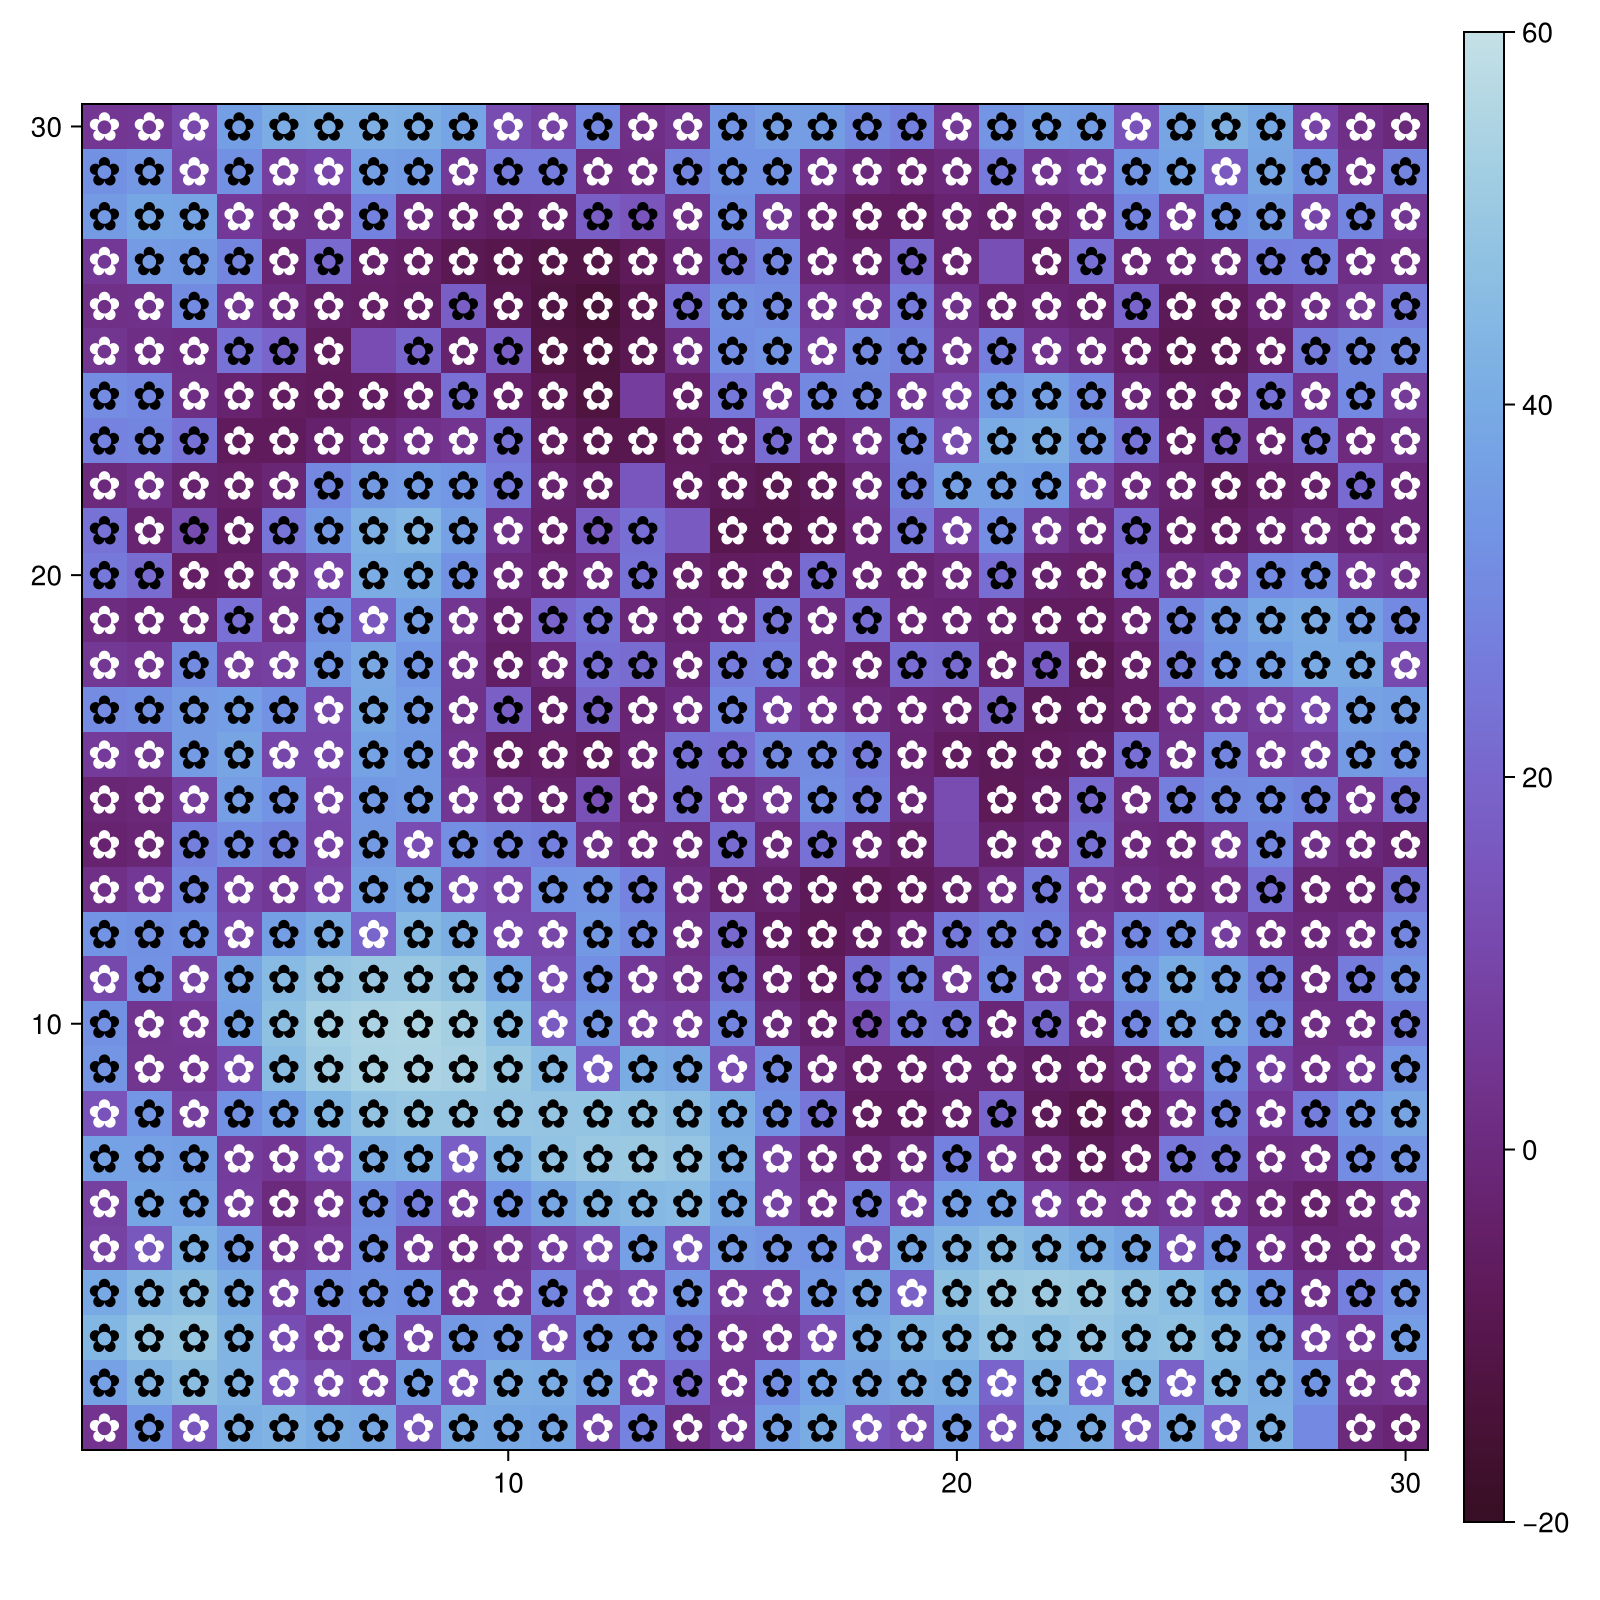
\includegraphics[width=0.7\textwidth,height=\textheight]{image/pic040.png}

}

\caption{\label{fig-005}Daisy\_step40}

\end{figure}%

Запустив файл и посмотрев на результаты, я преобразовала его в
литературный стиль(рис.~\ref{fig-006})

\begin{figure}

\centering{


\includegraphics[width=0.7\textwidth,height=\textheight]{image/pic9.png}

}

\caption{\label{fig-006}преобразования кода в литературный}

\end{figure}%

Я генерирую следующие файлы из литературного кода: чистый код, jupyter
notebook и документация в формате Quarto. После этого я проверяю, чтобы
убедиться, что все ячейки в файле jupyter notebook работают без
ошибок(рис.~\ref{fig-007})

\begin{figure}

\centering{


\includegraphics[width=0.7\textwidth,height=\textheight]{image/pic11.png}

}

\caption{\label{fig-007}проверка работы код}

\end{figure}%

\textbf{\emph{Ниже приведен код, результаты расчетов и графики для кода
в файле scripts/daisyworld.jl.qmd}}

\chapter{Базовая визуализация модели
Daisyworld}\label{ux431ux430ux437ux43eux432ux430ux44f-ux432ux438ux437ux443ux430ux43bux438ux437ux430ux446ux438ux44f-ux43cux43eux434ux435ux43bux438-daisyworld}

\section{Описание}\label{ux43eux43fux438ux441ux430ux43dux438ux435}

Этот скрипт демонстрирует базовую визуализацию модели Daisyworld в
разные моменты времени: начальное состояние (t=0), после 5 шагов и после
40 шагов моделирования.

\section{Подготовка
окружения}\label{ux43fux43eux434ux433ux43eux442ux43eux432ux43aux430-ux43eux43aux440ux443ux436ux435ux43dux438ux44f}

Активируем проект DrWatson и загружаем необходимые пакеты:

\begin{Shaded}
\begin{Highlighting}[]
\ImportTok{using} \BuiltInTok{DrWatson}
\PreprocessorTok{@quickactivate} \StringTok{"project"}

\ImportTok{using} \BuiltInTok{Agents}      \CommentTok{\# для агентного моделирования}
\ImportTok{using} \BuiltInTok{DataFrames}  \CommentTok{\# для работы с данными}
\ImportTok{using} \BuiltInTok{Plots}       \CommentTok{\# для визуализации (бэкенд)}
\end{Highlighting}
\end{Shaded}

\begin{verbatim}
┌ Warning: DrWatson could not find find a project file by recursively checking given `dir` and its parents. Returning `nothing` instead.
│ (given dir: /home/nelianjovu)
└ @ DrWatson ~/.julia/packages/DrWatson/2QF5p/src/project_setup.jl:84
\end{verbatim}

\section{Подключение
модели}\label{ux43fux43eux434ux43aux43bux44eux447ux435ux43dux438ux435-ux43cux43eux434ux435ux43bux438}

Подключаем файл с реализацией модели Daisyworld (предполагается, что он
находится в \texttt{src/daisyworld.jl})

\begin{Shaded}
\begin{Highlighting}[]
\FunctionTok{include}\NormalTok{(}\FunctionTok{srcdir}\NormalTok{(}\StringTok{"daisyworld.jl"}\NormalTok{))}
\end{Highlighting}
\end{Shaded}

\begin{verbatim}
daisyworld (generic function with 1 method)
\end{verbatim}

\section{Выбор бэкенда для
визуализации}\label{ux432ux44bux431ux43eux440-ux431ux44dux43aux435ux43dux434ux430-ux434ux43bux44f-ux432ux438ux437ux443ux430ux43bux438ux437ux430ux446ux438ux438}

Используем CairoMakie для высококачественной графики

\begin{Shaded}
\begin{Highlighting}[]
\ImportTok{using} \BuiltInTok{CairoMakie}
\end{Highlighting}
\end{Shaded}

\section{Создание
модели}\label{ux441ux43eux437ux434ux430ux43dux438ux435-ux43cux43eux434ux435ux43bux438}

Инициализируем мир Daisyworld с параметрами по умолчанию: - сетка 30×30
клеток - максимальный возраст маргариток 25 шагов - начальная доля белых
и чёрных маргариток по 20\%

\begin{Shaded}
\begin{Highlighting}[]
\NormalTok{model }\OperatorTok{=} \FunctionTok{daisyworld}\NormalTok{()}
\end{Highlighting}
\end{Shaded}

\begin{verbatim}
StandardABM with 360 agents of type Daisy
 agents container: Dict
 space: GridSpaceSingle with size (30, 30), metric=chebyshev, periodic=true
 scheduler: fastest
 properties: temperature, solar_luminosity, max_age, surface_albedo, ratio, solar_change, tick, scenario
\end{verbatim}

\section{Настройка
визуализации}\label{ux43dux430ux441ux442ux440ux43eux439ux43aux430-ux432ux438ux437ux443ux430ux43bux438ux437ux430ux446ux438ux438}

\subsection{Цвет
агентов}\label{ux446ux432ux435ux442-ux430ux433ux435ux43dux442ux43eux432}

Определяем функцию, которая возвращает цвет маргаритки в зависимости от
её типа: - чёрные маргаритки будут отображаться чёрным цветом - белые
маргаритки будут отображаться белым цветом

\begin{Shaded}
\begin{Highlighting}[]
\FunctionTok{daisycolor}\NormalTok{(a}\OperatorTok{::}\DataTypeTok{Daisy}\NormalTok{) }\OperatorTok{=}\NormalTok{ a.breed  }\CommentTok{\# :black или :white}
\end{Highlighting}
\end{Shaded}

\begin{verbatim}
daisycolor (generic function with 1 method)
\end{verbatim}

\subsection{Параметры
графика}\label{ux43fux430ux440ux430ux43cux435ux442ux440ux44b-ux433ux440ux430ux444ux438ux43aux430}

Настраиваем внешний вид визуализации: - \texttt{agent\_color} - цвет
агентов (определён выше) - \texttt{agent\_size} - размер маркеров
агентов - \texttt{agent\_marker} - символ для отображения агентов (✿ -
цветок) - \texttt{heatarray} - данные для тепловой карты (температура) -
\texttt{heatkwargs} - дополнительные параметры тепловой карты

\begin{Shaded}
\begin{Highlighting}[]
\NormalTok{plotkwargs }\OperatorTok{=}\NormalTok{ (}
\NormalTok{    agent\_color }\OperatorTok{=}\NormalTok{ daisycolor,}
\NormalTok{    agent\_size }\OperatorTok{=} \FloatTok{20}\NormalTok{,}
\NormalTok{    agent\_marker }\OperatorTok{=} \CharTok{\textquotesingle{}✿\textquotesingle{}}\NormalTok{,}
\NormalTok{    heatarray }\OperatorTok{=} \OperatorTok{:}\NormalTok{temperature,}
\NormalTok{    heatkwargs }\OperatorTok{=}\NormalTok{ (colorrange }\OperatorTok{=}\NormalTok{ (}\OperatorTok{{-}}\FloatTok{20}\NormalTok{, }\FloatTok{60}\NormalTok{),),}
\NormalTok{)}
\end{Highlighting}
\end{Shaded}

\begin{verbatim}
(agent_color = daisycolor, agent_size = 20, agent_marker = '✿', heatarray = :temperature, heatkwargs = (colorrange = (-20, 60),))
\end{verbatim}

\section{Визуализация начального состояния (t =
0)}\label{ux432ux438ux437ux443ux430ux43bux438ux437ux430ux446ux438ux44f-ux43dux430ux447ux430ux43bux44cux43dux43eux433ux43e-ux441ux43eux441ux442ux43eux44fux43dux438ux44f-t-0}

Создаём график начального состояния модели. На графике отображаются: -
тепловая карта температуры поверхности - маргаритки (чёрные и белые
символы)

\begin{Shaded}
\begin{Highlighting}[]
\FunctionTok{println}\NormalTok{(}\StringTok{"Визуализация начального состояния (t = 0)"}\NormalTok{)}
\NormalTok{plt1, \_ }\OperatorTok{=} \FunctionTok{abmplot}\NormalTok{(model; plotkwargs}\OperatorTok{...}\NormalTok{)}
\NormalTok{plt1}
\end{Highlighting}
\end{Shaded}

\begin{verbatim}
Визуализация начального состояния (t = 0)
\end{verbatim}

\begin{verbatim}
┌ Warning: Found `resolution` in the theme when creating a `Scene`. The `resolution` keyword for `Scene`s and `Figure`s has been deprecated. Use `Figure(; size = ...` or `Scene(; size = ...)` instead, which better reflects that this is a unitless size and not a pixel resolution. The key could also come from `set_theme!` calls or related theming functions.
└ @ Makie ~/.julia/packages/Makie/kJl0u/src/scenes.jl:264
\end{verbatim}

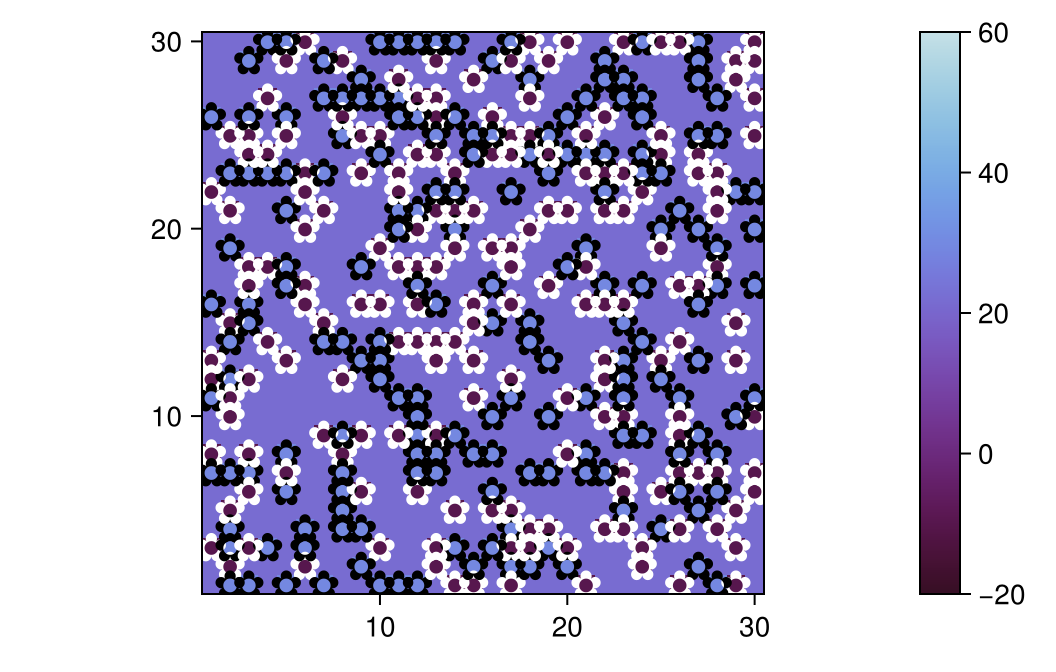
\includegraphics{simmod-lab03-report (Нджову Нелиа)_files/figure-pdf/cell-9-output-3.png}

\section{Моделирование 5
шагов}\label{ux43cux43eux434ux435ux43bux438ux440ux43eux432ux430ux43dux438ux435-5-ux448ux430ux433ux43eux432}

Выполняем 5 шагов моделирования

\begin{Shaded}
\begin{Highlighting}[]
\FunctionTok{step!}\NormalTok{(model, }\FloatTok{5}\NormalTok{)}
\FunctionTok{println}\NormalTok{(}\StringTok{"Визуализация после 5 шагов"}\NormalTok{)}
\NormalTok{plt2, \_ }\OperatorTok{=} \FunctionTok{abmplot}\NormalTok{(model; heatarray }\OperatorTok{=}\NormalTok{ model.temperature, plotkwargs}\OperatorTok{...}\NormalTok{)}
\NormalTok{plt2}
\end{Highlighting}
\end{Shaded}

\begin{verbatim}
Визуализация после 5 шагов
\end{verbatim}

\begin{verbatim}
┌ Warning: Found `resolution` in the theme when creating a `Scene`. The `resolution` keyword for `Scene`s and `Figure`s has been deprecated. Use `Figure(; size = ...` or `Scene(; size = ...)` instead, which better reflects that this is a unitless size and not a pixel resolution. The key could also come from `set_theme!` calls or related theming functions.
└ @ Makie ~/.julia/packages/Makie/kJl0u/src/scenes.jl:264
\end{verbatim}

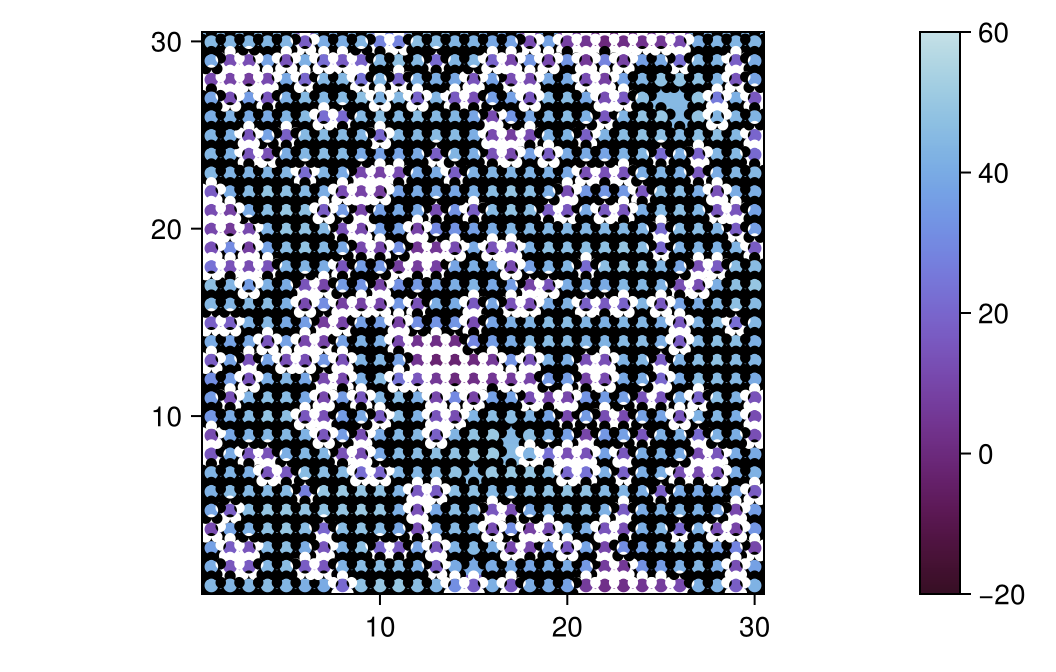
\includegraphics{simmod-lab03-report (Нджову Нелиа)_files/figure-pdf/cell-10-output-3.png}

\section{Моделирование до 40
шагов}\label{ux43cux43eux434ux435ux43bux438ux440ux43eux432ux430ux43dux438ux435-ux434ux43e-40-ux448ux430ux433ux43eux432}

Выполняем ещё 35 шагов (всего станет 40)

\begin{Shaded}
\begin{Highlighting}[]
\FunctionTok{step!}\NormalTok{(model, }\FloatTok{35}\NormalTok{)}
\FunctionTok{println}\NormalTok{(}\StringTok{"Визуализация после 40 шагов"}\NormalTok{)}
\NormalTok{plt3, \_ }\OperatorTok{=} \FunctionTok{abmplot}\NormalTok{(model; heatarray }\OperatorTok{=}\NormalTok{ model.temperature, plotkwargs}\OperatorTok{...}\NormalTok{)}
\NormalTok{plt3}
\end{Highlighting}
\end{Shaded}

\begin{verbatim}
Визуализация после 40 шагов
\end{verbatim}

\begin{verbatim}
┌ Warning: Found `resolution` in the theme when creating a `Scene`. The `resolution` keyword for `Scene`s and `Figure`s has been deprecated. Use `Figure(; size = ...` or `Scene(; size = ...)` instead, which better reflects that this is a unitless size and not a pixel resolution. The key could also come from `set_theme!` calls or related theming functions.
└ @ Makie ~/.julia/packages/Makie/kJl0u/src/scenes.jl:264
\end{verbatim}

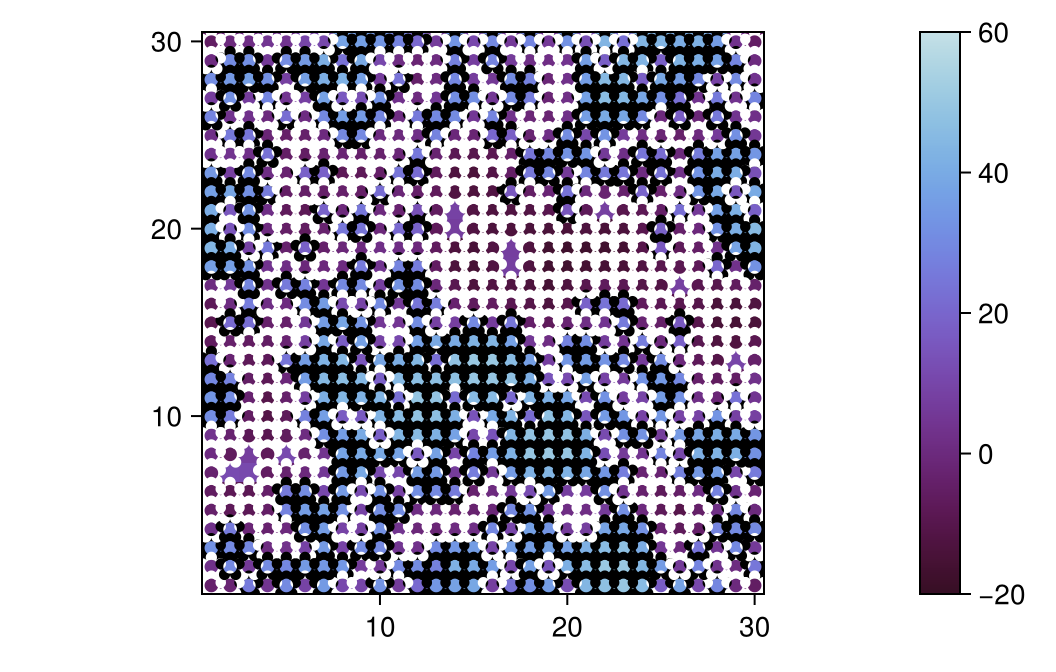
\includegraphics{simmod-lab03-report (Нджову Нелиа)_files/figure-pdf/cell-11-output-3.png}

\section{Итог}\label{ux438ux442ux43eux433}

\begin{Shaded}
\begin{Highlighting}[]
\FunctionTok{println}\NormalTok{(}\StringTok{"}\SpecialCharTok{\textbackslash{}n}\StringTok{Все графики сохранены в каталоге: "}\NormalTok{, }\FunctionTok{plotsdir}\NormalTok{())}
\FunctionTok{println}\NormalTok{(}\StringTok{"   {-} daisy\_step001.png (начальное состояние)"}\NormalTok{)}
\FunctionTok{println}\NormalTok{(}\StringTok{"   {-} daisy\_step005.png (после 5 шагов)"}\NormalTok{)}
\FunctionTok{println}\NormalTok{(}\StringTok{"   {-} daisy\_step040.png (после 40 шагов)"}\NormalTok{)}
\end{Highlighting}
\end{Shaded}

\begin{verbatim}

Все графики сохранены в каталоге: /home/nelianjovu/work/study/2026-1/2026-1==study--simulationmod/2026-1--study--simulationmod/labs/lab03/project/plots
   - daisy_step001.png (начальное состояние)
   - daisy_step005.png (после 5 шагов)
   - daisy_step040.png (после 40 шагов)
\end{verbatim}

Сохраняем график в каталог \texttt{plots} проекта

\begin{Shaded}
\begin{Highlighting}[]
\FunctionTok{save}\NormalTok{(}\FunctionTok{plotsdir}\NormalTok{(}\StringTok{"daisy\_step001.png"}\NormalTok{), plt1)}
\FunctionTok{save}\NormalTok{(}\FunctionTok{plotsdir}\NormalTok{(}\StringTok{"daisy\_step005.png"}\NormalTok{), plt2)}
\FunctionTok{save}\NormalTok{(}\FunctionTok{plotsdir}\NormalTok{(}\StringTok{"daisy\_step040.png"}\NormalTok{), plt3)}
\end{Highlighting}
\end{Shaded}

\section{3. Анимация
модели}\label{ux430ux43dux438ux43cux430ux446ux438ux44f-ux43cux43eux434ux435ux43bux438}

Я создала файл scripts/daisyworld-animate.jl и скопировала скрипт код,
который мне дали и запускала его.Этот скрипт создает анимационный
видеоролик о модели Daisyworld(рис.~\ref{fig-008})

\begin{figure}

\centering{


\includegraphics[width=0.7\textwidth,height=\textheight]{image/pic13.png}

}

\caption{\label{fig-008}Анимация модели}

\end{figure}%

\emph{На видео показано, как система Daisyworld эволюционирует с
течением времени. Вначале (t=0-50) маргаритки разбросаны случайным
образом, а температура по всей планете довольно однородна. В процессе
моделирования (t=50-200) вы можете отчетливо видеть, как появляются
узоры --- черные ромашки создают теплые пятна, поглощая тепло, в то
время как белые ромашки образуют холодные пятна, отражая солнечный свет.
К тому времени, когда система достигает динамического равновесия
(t=200+), формируются устойчивые структуры, в которых черные и белые
ромашки чередуются по всей сетке, а температура остается
сбалансированной в пределах оптимального диапазона для роста. Когда
черных ромашек становится больше, белых ромашек становится меньше, и
наоборот. Это очень похоже на результаты для сценария daisyworld, только
здесь мы видим, как меняются шаблоны}

\section{4. Динамика числа
маргариток}\label{ux434ux438ux43dux430ux43cux438ux43aux430-ux447ux438ux441ux43bux430-ux43cux430ux440ux433ux430ux440ux438ux442ux43eux43a}

Я создала файл scripts/daisyworld-count.jl и скопировала скрипт код,
который мне дали и запускала его. Этот скрипт анализирует динамику
популяции, отслеживая, как меняется количество черных и белых маргариток
на протяжении 1000 шагов моделирования(рис.~\ref{fig-009})

\begin{figure}

\centering{


\includegraphics[width=0.7\textwidth,height=\textheight]{image/pic14.png}

}

\caption{\label{fig-009}запуск код}

\end{figure}%

На графике показано, как популяции черной и белой маргариток меняются на
протяжении 1000 шагов. Вначале обе популяции быстро растут по сравнению
с их первоначальной численностью. Затем, примерно через 200 шагов, мы
начинаем наблюдать регулярные подъемы и спады, когда черные ромашки
поднимаются, белые опускаются, а затем происходит обратное. Эта
закономерность сохраняется на протяжении всего моделирования. Это
происходит из-за обратной связи: когда черных маргариток становится
больше, они согревают планету, что затем помогает расти белым
маргариткам; когда белых маргариток становится больше, они охлаждают
планету, что помогает расти черным маргариткам(рис.~\ref{fig-010})

\begin{figure}

\centering{


\includegraphics[width=0.7\textwidth,height=\textheight]{image/pic15.png}

}

\caption{\label{fig-010}График изменения числа маргариток}

\end{figure}%

Запустив файл и посмотрев на результаты, я преобразовала его в
литературный стиль(рис.~\ref{fig-011})

\begin{figure}

\centering{


\includegraphics[width=0.7\textwidth,height=\textheight]{image/pic17.png}

}

\caption{\label{fig-011}преобразования кода в литературный}

\end{figure}%

Я генерирую следующие файлы из литературного кода: чистый код, jupyter
notebook и документация в формате Quarto. После этого я проверяю, чтобы
убедиться, что все ячейки в файле jupyter notebook работают без
ошибок(рис.~\ref{fig-012})

\begin{figure}

\centering{


\includegraphics[width=0.7\textwidth,height=\textheight]{image/pic16.png}

}

\caption{\label{fig-012}проверка работы код}

\end{figure}%

\textbf{\emph{Ниже приведен код, результаты расчетов и графики для кода
в файле scripts/daisyworld-count.jl.qmd}}

\chapter{Анализ динамики численности маргариток в модели
Daisyworld}\label{ux430ux43dux430ux43bux438ux437-ux434ux438ux43dux430ux43cux438ux43aux438-ux447ux438ux441ux43bux435ux43dux43dux43eux441ux442ux438-ux43cux430ux440ux433ux430ux440ux438ux442ux43eux43a-ux432-ux43cux43eux434ux435ux43bux438-daisyworld}

\section{Описание}\label{ux43eux43fux438ux441ux430ux43dux438ux435-1}

Этот скрипт анализирует изменение количества чёрных и белых маргариток
во времени на протяжении 1000 шагов моделирования. Строится график
динамики численности обоих типов маргариток.

\section{Подготовка
окружения}\label{ux43fux43eux434ux433ux43eux442ux43eux432ux43aux430-ux43eux43aux440ux443ux436ux435ux43dux438ux44f-1}

Активируем проект DrWatson и загружаем необходимые пакеты:

\begin{Shaded}
\begin{Highlighting}[]
\ImportTok{using} \BuiltInTok{DrWatson}
\PreprocessorTok{@quickactivate} \StringTok{"project"}
\ImportTok{using} \BuiltInTok{Agents}      \CommentTok{\# для агентного моделирования}
\ImportTok{using} \BuiltInTok{DataFrames}  \CommentTok{\# для работы с данными}
\ImportTok{using} \BuiltInTok{Plots}       \CommentTok{\# базовый бэкенд для графиков}
\end{Highlighting}
\end{Shaded}

\begin{verbatim}
┌ Warning: DrWatson could not find find a project file by recursively checking given `dir` and its parents. Returning `nothing` instead.
│ (given dir: /home/nelianjovu)
└ @ DrWatson ~/.julia/packages/DrWatson/2QF5p/src/project_setup.jl:84
\end{verbatim}

\section{Подключение
модели}\label{ux43fux43eux434ux43aux43bux44eux447ux435ux43dux438ux435-ux43cux43eux434ux435ux43bux438-1}

Подключаем файл с реализацией модели Daisyworld (находится в
\texttt{src/daisyworld.jl})

\begin{Shaded}
\begin{Highlighting}[]
\FunctionTok{include}\NormalTok{(}\FunctionTok{srcdir}\NormalTok{(}\StringTok{"daisyworld.jl"}\NormalTok{))}

\ImportTok{using} \BuiltInTok{CairoMakie}  \CommentTok{\# для высококачественной визуализации}
\end{Highlighting}
\end{Shaded}

\section{Определение функций для сбора
данных}\label{ux43eux43fux440ux435ux434ux435ux43bux435ux43dux438ux435-ux444ux443ux43dux43aux446ux438ux439-ux434ux43bux44f-ux441ux431ux43eux440ux430-ux434ux430ux43dux43dux44bux445}

Создаём функции-предикаты для идентификации типа маргариток:

\begin{Shaded}
\begin{Highlighting}[]
\FunctionTok{black}\NormalTok{(a}\OperatorTok{::}\DataTypeTok{Daisy}\NormalTok{) }\OperatorTok{=}\NormalTok{ a.breed }\OperatorTok{==} \OperatorTok{:}\NormalTok{black}
\FunctionTok{white}\NormalTok{(a}\OperatorTok{::}\DataTypeTok{Daisy}\NormalTok{) }\OperatorTok{=}\NormalTok{ a.breed }\OperatorTok{==} \OperatorTok{:}\NormalTok{white}
\end{Highlighting}
\end{Shaded}

\begin{verbatim}
white (generic function with 1 method)
\end{verbatim}

\section{Настройка сбора
данных}\label{ux43dux430ux441ux442ux440ux43eux439ux43aux430-ux441ux431ux43eux440ux430-ux434ux430ux43dux43dux44bux445}

Указываем, какие данные собирать в процессе моделирования: - для чёрных
маргариток: подсчёт количества - для белых маргариток: подсчёт
количества

\begin{Shaded}
\begin{Highlighting}[]
\NormalTok{adata }\OperatorTok{=}\NormalTok{ [(black, count), (white, count)]}
\end{Highlighting}
\end{Shaded}

\begin{verbatim}
2-element Vector{Tuple{Function, typeof(count)}}:
 (black, count)
 (white, count)
\end{verbatim}

\section{Создание
модели}\label{ux441ux43eux437ux434ux430ux43dux438ux435-ux43cux43eux434ux435ux43bux438-1}

Инициализируем мир Daisyworld с начальной светимостью 1.0:

\begin{Shaded}
\begin{Highlighting}[]
\NormalTok{model }\OperatorTok{=} \FunctionTok{daisyworld}\NormalTok{(; solar\_luminosity }\OperatorTok{=} \FloatTok{1.0}\NormalTok{)}
\end{Highlighting}
\end{Shaded}

\begin{verbatim}
StandardABM with 360 agents of type Daisy
 agents container: Dict
 space: GridSpaceSingle with size (30, 30), metric=chebyshev, periodic=true
 scheduler: fastest
 properties: temperature, solar_luminosity, max_age, surface_albedo, ratio, solar_change, tick, scenario
\end{verbatim}

\section{Запуск
моделирования}\label{ux437ux430ux43fux443ux441ux43a-ux43cux43eux434ux435ux43bux438ux440ux43eux432ux430ux43dux438ux44f}

Выполняем 1000 шагов моделирования и собираем данные о численности
маргариток на каждом шаге:

\begin{Shaded}
\begin{Highlighting}[]
\FunctionTok{println}\NormalTok{(}\StringTok{"🔄 Запуск моделирования на 1000 шагов..."}\NormalTok{)}
\NormalTok{agent\_df, model\_df }\OperatorTok{=} \FunctionTok{run!}\NormalTok{(model, }\FloatTok{1000}\NormalTok{; adata)}
\end{Highlighting}
\end{Shaded}

\begin{verbatim}
🔄 Запуск моделирования на 1000 шагов...
\end{verbatim}

\begin{verbatim}
(1001×3 DataFrame
  Row │ time   count_black  count_white 
      │ Int64  Int64        Int64       
──────┼─────────────────────────────────
    1 │     0          180          180
    2 │     1          374          167
    3 │     2          516          207
    4 │     3          564          280
    5 │     4          564          312
    6 │     5          557          335
    7 │     6          559          339
    8 │     7          560          337
    9 │     8          559          339
   10 │     9          553          345
   11 │    10          552          346
  ⋮   │   ⋮         ⋮            ⋮
  992 │   991          498          400
  993 │   992          495          402
  994 │   993          492          404
  995 │   994          490          405
  996 │   995          485          408
  997 │   996          486          408
  998 │   997          489          407
  999 │   998          496          399
 1000 │   999          508          386
 1001 │  1000          513          382
                        980 rows omitted, 0×0 DataFrame)
\end{verbatim}

\section{Визуализация
результатов}\label{ux432ux438ux437ux443ux430ux43bux438ux437ux430ux446ux438ux44f-ux440ux435ux437ux443ux43bux44cux442ux430ux442ux43eux432}

Создаём график динамики численности маргариток с помощью CairoMakie:

Создаём фигуру размером 600×400 пикселей

\begin{Shaded}
\begin{Highlighting}[]
\NormalTok{figure }\OperatorTok{=} \FunctionTok{Figure}\NormalTok{(size }\OperatorTok{=}\NormalTok{ (}\FloatTok{600}\NormalTok{, }\FloatTok{400}\NormalTok{))}
\end{Highlighting}
\end{Shaded}

\begin{verbatim}
┌ Warning: Found `resolution` in the theme when creating a `Scene`. The `resolution` keyword for `Scene`s and `Figure`s has been deprecated. Use `Figure(; size = ...` or `Scene(; size = ...)` instead, which better reflects that this is a unitless size and not a pixel resolution. The key could also come from `set_theme!` calls or related theming functions.
└ @ Makie ~/.julia/packages/Makie/kJl0u/src/scenes.jl:264
\end{verbatim}


\includegraphics{simmod-lab03-report (Нджову Нелиа)_files/figure-pdf/cell-20-output-2.png}

Создаём оси с подписями

\begin{Shaded}
\begin{Highlighting}[]
\NormalTok{ax }\OperatorTok{=} \FunctionTok{Axis}\NormalTok{(figure[}\FloatTok{1}\NormalTok{, }\FloatTok{1}\NormalTok{],}
\NormalTok{          xlabel }\OperatorTok{=} \StringTok{"Время (шаги)"}\NormalTok{,}
\NormalTok{          ylabel }\OperatorTok{=} \StringTok{"Количество маргариток"}\NormalTok{,}
\NormalTok{          title }\OperatorTok{=} \StringTok{"Динамика численности маргариток в модели Daisyworld"}\NormalTok{)}
\end{Highlighting}
\end{Shaded}

\begin{verbatim}
Axis with 0 plots:
\end{verbatim}

Строим линии для чёрных и белых маргариток

\begin{Shaded}
\begin{Highlighting}[]
\NormalTok{black\_line }\OperatorTok{=} \FunctionTok{lines!}\NormalTok{(ax, agent\_df[!, }\OperatorTok{:}\NormalTok{time], agent\_df[!, }\OperatorTok{:}\NormalTok{count\_black],}
\NormalTok{                    color }\OperatorTok{=} \OperatorTok{:}\NormalTok{black, linewidth }\OperatorTok{=} \FloatTok{2}\NormalTok{, label }\OperatorTok{=} \StringTok{"Чёрные"}\NormalTok{)}
\NormalTok{white\_line }\OperatorTok{=} \FunctionTok{lines!}\NormalTok{(ax, agent\_df[!, }\OperatorTok{:}\NormalTok{time], agent\_df[!, }\OperatorTok{:}\NormalTok{count\_white],}
\NormalTok{                    color }\OperatorTok{=} \OperatorTok{:}\NormalTok{orange, linewidth }\OperatorTok{=} \FloatTok{2}\NormalTok{, label }\OperatorTok{=} \StringTok{"Белые"}\NormalTok{)}
\end{Highlighting}
\end{Shaded}

\begin{verbatim}
Lines{Tuple{Vector{Point{2, Float64}}}}
\end{verbatim}

Добавляем легенду

\begin{Shaded}
\begin{Highlighting}[]
\FunctionTok{Legend}\NormalTok{(figure[}\FloatTok{1}\NormalTok{, }\FloatTok{2}\NormalTok{], [black\_line, white\_line], [}\StringTok{"Чёрные"}\NormalTok{, }\StringTok{"Белые"}\NormalTok{], labelsize }\OperatorTok{=} \FloatTok{12}\NormalTok{)}

\FunctionTok{display}\NormalTok{(figure)}
\end{Highlighting}
\end{Shaded}


\includegraphics{simmod-lab03-report (Нджову Нелиа)_files/figure-pdf/cell-23-output-1.png}

\begin{verbatim}
CairoMakie.Screen{IMAGE}
\end{verbatim}

\section{Сохранение
графика}\label{ux441ux43eux445ux440ux430ux43dux435ux43dux438ux435-ux433ux440ux430ux444ux438ux43aux430}

Сохраняем полученный график в каталог \texttt{plots} проекта:

\begin{Shaded}
\begin{Highlighting}[]
\FunctionTok{save}\NormalTok{(}\FunctionTok{plotsdir}\NormalTok{(}\StringTok{"daisy\_count.png"}\NormalTok{), figure)}
\FunctionTok{println}\NormalTok{(}\StringTok{"График сохранён: "}\NormalTok{, }\FunctionTok{plotsdir}\NormalTok{(}\StringTok{"daisy\_count.png"}\NormalTok{))}
\end{Highlighting}
\end{Shaded}

\begin{verbatim}
График сохранён: /home/nelianjovu/work/study/2026-1/2026-1==study--simulationmod/2026-1--study--simulationmod/labs/lab03/project/plots/daisy_count.png
\end{verbatim}

\section{5 Динамика
модели}\label{ux434ux438ux43dux430ux43cux438ux43aux430-ux43cux43eux434ux435ux43bux438}

Я создала файл scripts/daisyworld-luminosity.jl и скопировала скрипт
код, который мне дали и запускала его. Этот сценарий анализирует, как
изменение яркости солнца влияет на систему Daisyworld, используя
сценарий :ramp(рис.~\ref{fig-013})

\begin{figure}

\centering{


\includegraphics[width=0.7\textwidth,height=\textheight]{image/pic18.png}

}

\caption{\label{fig-013}запуск код}

\end{figure}%

На графике показано, как Daisyworld реагирует, когда яркость солнца
увеличивается, а затем уменьшается. На графике вверху вы можете видеть,
что популяции черных и белых маргариток меняются по мере изменения
солнца: когда яркость увеличивается, белые маргаритки (синяя линия)
становятся более распространенными, потому что они отражают тепло и
помогают охлаждать планету; когда яркость уменьшается, преобладают
черные маргаритки (красная линия), потому что они поглощают тепло и
разогреть обстановку. График в середине показывает температуру, которая
остается довольно стабильной, несмотря на то, что на графике внизу
солнце сильно меняется. Маргаритки защищают планету от резких перепадов
температуры. Кроме того, если мы присмотримся повнимательнее, то увидим,
что система ведет себя не совсем одинаково на подъеме и на
спаде(рис.~\ref{fig-014})

\begin{figure}

\centering{


\includegraphics[width=0.7\textwidth,height=\textheight]{image/pic19.png}

}

\caption{\label{fig-014}Динамика модели}

\end{figure}%

Запустив файл и посмотрев на результаты, я преобразовала его в
литературный стиль(рис.~\ref{fig-015})

\begin{figure}

\centering{


\includegraphics[width=0.7\textwidth,height=\textheight]{image/pic21.png}

}

\caption{\label{fig-015}преобразования кода в литературный}

\end{figure}%

Я генерирую следующие файлы из литературного кода: чистый код, jupyter
notebook и документация в формате Quarto. После этого я проверяю, чтобы
убедиться, что все ячейки в файле jupyter notebook работают без
ошибок(рис.~\ref{fig-016})

\begin{figure}

\centering{


\includegraphics[width=0.7\textwidth,height=\textheight]{image/pic22.png}

}

\caption{\label{fig-016}проверка работы код}

\end{figure}%

\textbf{\emph{Ниже приведен код, результаты расчетов и графики для кода
в файле scripts/daisyworld-luminosity.jl.qmd}}

\chapter{Анализ влияния солнечной активности на модель
Daisyworld}\label{ux430ux43dux430ux43bux438ux437-ux432ux43bux438ux44fux43dux438ux44f-ux441ux43eux43bux43dux435ux447ux43dux43eux439-ux430ux43aux442ux438ux432ux43dux43eux441ux442ux438-ux43dux430-ux43cux43eux434ux435ux43bux44c-daisyworld}

\section{Описание}\label{ux43eux43fux438ux441ux430ux43dux438ux435-2}

Этот скрипт исследует влияние изменения солнечной активности на динамику
модели Daisyworld. Анализируются три взаимосвязанных показателя: -
численность чёрных и белых маргариток - средняя температура поверхности
планеты - уровень солнечной светимости

Модель запускается со сценарием \texttt{:ramp}, который имитирует
постепенное увеличение, а затем уменьшение солнечной активности.

\section{Подготовка
окружения}\label{ux43fux43eux434ux433ux43eux442ux43eux432ux43aux430-ux43eux43aux440ux443ux436ux435ux43dux438ux44f-2}

Активируем проект DrWatson и загружаем необходимые пакеты:

\begin{Shaded}
\begin{Highlighting}[]
\ImportTok{using} \BuiltInTok{DrWatson}
\PreprocessorTok{@quickactivate} \StringTok{"project"}
\ImportTok{using} \BuiltInTok{Agents}      \CommentTok{\# для агентного моделирования}
\ImportTok{using} \BuiltInTok{DataFrames}  \CommentTok{\# для работы с данными}
\ImportTok{using} \BuiltInTok{Plots}       \CommentTok{\# базовый бэкенд для графиков}
\ImportTok{using} \BuiltInTok{CairoMakie}  \CommentTok{\# для высококачественной визуализации}
\end{Highlighting}
\end{Shaded}

\begin{verbatim}
┌ Warning: DrWatson could not find find a project file by recursively checking given `dir` and its parents. Returning `nothing` instead.
│ (given dir: /home/nelianjovu)
└ @ DrWatson ~/.julia/packages/DrWatson/2QF5p/src/project_setup.jl:84
\end{verbatim}

\section{Подключение
модели}\label{ux43fux43eux434ux43aux43bux44eux447ux435ux43dux438ux435-ux43cux43eux434ux435ux43bux438-2}

Подключаем файл с реализацией модели Daisyworld (находится в
\texttt{src/daisyworld.jl})

\begin{Shaded}
\begin{Highlighting}[]
\FunctionTok{include}\NormalTok{(}\FunctionTok{srcdir}\NormalTok{(}\StringTok{"daisyworld.jl"}\NormalTok{))}

\ImportTok{using} \BuiltInTok{CairoMakie}  \CommentTok{\# для высококачественной визуализации}
\end{Highlighting}
\end{Shaded}

\section{Определение функций для сбора
данных}\label{ux43eux43fux440ux435ux434ux435ux43bux435ux43dux438ux435-ux444ux443ux43dux43aux446ux438ux439-ux434ux43bux44f-ux441ux431ux43eux440ux430-ux434ux430ux43dux43dux44bux445-1}

Создаём функции-предикаты для идентификации типа маргариток:

\begin{Shaded}
\begin{Highlighting}[]
\FunctionTok{black}\NormalTok{(a}\OperatorTok{::}\DataTypeTok{Daisy}\NormalTok{) }\OperatorTok{=}\NormalTok{ a.breed }\OperatorTok{==} \OperatorTok{:}\NormalTok{black}
\FunctionTok{white}\NormalTok{(a}\OperatorTok{::}\DataTypeTok{Daisy}\NormalTok{) }\OperatorTok{=}\NormalTok{ a.breed }\OperatorTok{==} \OperatorTok{:}\NormalTok{white}
\end{Highlighting}
\end{Shaded}

\begin{verbatim}
white (generic function with 1 method)
\end{verbatim}

\section{Настройка сбора
данных}\label{ux43dux430ux441ux442ux440ux43eux439ux43aux430-ux441ux431ux43eux440ux430-ux434ux430ux43dux43dux44bux445-1}

Указываем, какие данные собирать в процессе моделирования: - для
агентов: подсчёт чёрных и белых маргариток - для модели: средняя
температура и уровень светимости

\begin{Shaded}
\begin{Highlighting}[]
\NormalTok{adata }\OperatorTok{=}\NormalTok{ [(black, count), (white, count)]  }\CommentTok{\# данные об агентах}
\end{Highlighting}
\end{Shaded}

\begin{verbatim}
2-element Vector{Tuple{Function, typeof(count)}}:
 (black, count)
 (white, count)
\end{verbatim}

Функция для вычисления средней температуры

\begin{Shaded}
\begin{Highlighting}[]
\FunctionTok{temperature}\NormalTok{(model) }\OperatorTok{=}\NormalTok{ StatsBase.}\FunctionTok{mean}\NormalTok{(model.temperature)}
\NormalTok{mdata }\OperatorTok{=}\NormalTok{ [temperature, }\OperatorTok{:}\NormalTok{solar\_luminosity]  }\CommentTok{\# данные о модели}
\end{Highlighting}
\end{Shaded}

\begin{verbatim}
2-element Vector{Any}:
 temperature (generic function with 1 method)
 :solar_luminosity
\end{verbatim}

\section{Создание
модели}\label{ux441ux43eux437ux434ux430ux43dux438ux435-ux43cux43eux434ux435ux43bux438-2}

Инициализируем мир Daisywood со сценарием изменения светимости
\texttt{:ramp}: - начальная светимость: 1.0 - сценарий: :ramp
(светимость сначала растёт, потом падает)

\begin{Shaded}
\begin{Highlighting}[]
\FunctionTok{println}\NormalTok{(}\StringTok{"Создание модели Daisyworld со сценарием :ramp..."}\NormalTok{)}
\NormalTok{model }\OperatorTok{=} \FunctionTok{daisyworld}\NormalTok{(; solar\_luminosity }\OperatorTok{=} \FloatTok{1.0}\NormalTok{, scenario }\OperatorTok{=} \OperatorTok{:}\NormalTok{ramp)}
\end{Highlighting}
\end{Shaded}

\begin{verbatim}
Создание модели Daisyworld со сценарием :ramp...
\end{verbatim}

\begin{verbatim}
StandardABM with 360 agents of type Daisy
 agents container: Dict
 space: GridSpaceSingle with size (30, 30), metric=chebyshev, periodic=true
 scheduler: fastest
 properties: temperature, solar_luminosity, max_age, surface_albedo, ratio, solar_change, tick, scenario
\end{verbatim}

\section{Запуск
моделирования}\label{ux437ux430ux43fux443ux441ux43a-ux43cux43eux434ux435ux43bux438ux440ux43eux432ux430ux43dux438ux44f-1}

Выполняем 1000 шагов моделирования и собираем данные:

\begin{Shaded}
\begin{Highlighting}[]
\FunctionTok{println}\NormalTok{(}\StringTok{"Запуск моделирования на 1000 шагов..."}\NormalTok{)}
\NormalTok{agent\_df, model\_df }\OperatorTok{=} \FunctionTok{run!}\NormalTok{(model, }\FloatTok{1000}\NormalTok{; adata }\OperatorTok{=}\NormalTok{ adata, mdata }\OperatorTok{=}\NormalTok{ mdata)}

\FunctionTok{println}\NormalTok{(}\StringTok{"Моделирование завершено"}\NormalTok{)}
\FunctionTok{println}\NormalTok{(}\StringTok{"   {-} Собрано }\SpecialCharTok{$}\NormalTok{(}\FunctionTok{nrow}\NormalTok{(agent\_df))}\StringTok{ записей о популяциях"}\NormalTok{)}
\FunctionTok{println}\NormalTok{(}\StringTok{"   {-} Собрано }\SpecialCharTok{$}\NormalTok{(}\FunctionTok{nrow}\NormalTok{(model\_df))}\StringTok{ записей о состоянии модели"}\NormalTok{)}
\end{Highlighting}
\end{Shaded}

\begin{verbatim}
Запуск моделирования на 1000 шагов...
Моделирование завершено
   - Собрано 1001 записей о популяциях
   - Собрано 1001 записей о состоянии модели
\end{verbatim}

\section{Создание комплексной
визуализации}\label{ux441ux43eux437ux434ux430ux43dux438ux435-ux43aux43eux43cux43fux43bux435ux43aux441ux43dux43eux439-ux432ux438ux437ux443ux430ux43bux438ux437ux430ux446ux438ux438}

Создаём фигуру с тремя графиками, расположенными вертикально: 1.
Динамика численности маргариток 2. Изменение средней температуры 3.
Изменение солнечной светимости

Создаём фигуру размером 600×600 пикселей

\begin{Shaded}
\begin{Highlighting}[]
\NormalTok{figure }\OperatorTok{=}\NormalTok{ CairoMakie.}\FunctionTok{Figure}\NormalTok{(size }\OperatorTok{=}\NormalTok{ (}\FloatTok{600}\NormalTok{, }\FloatTok{600}\NormalTok{))}
\end{Highlighting}
\end{Shaded}

\begin{verbatim}
┌ Warning: Found `resolution` in the theme when creating a `Scene`. The `resolution` keyword for `Scene`s and `Figure`s has been deprecated. Use `Figure(; size = ...` or `Scene(; size = ...)` instead, which better reflects that this is a unitless size and not a pixel resolution. The key could also come from `set_theme!` calls or related theming functions.
└ @ Makie ~/.julia/packages/Makie/kJl0u/src/scenes.jl:264
\end{verbatim}


\includegraphics{simmod-lab03-report (Нджову Нелиа)_files/figure-pdf/cell-32-output-2.png}

\subsection{График 1: Динамика численности
маргариток}\label{ux433ux440ux430ux444ux438ux43a-1-ux434ux438ux43dux430ux43cux438ux43aux430-ux447ux438ux441ux43bux435ux43dux43dux43eux441ux442ux438-ux43cux430ux440ux433ux430ux440ux438ux442ux43eux43a}

\begin{Shaded}
\begin{Highlighting}[]
\NormalTok{ax1 }\OperatorTok{=} \FunctionTok{Axis}\NormalTok{(figure[}\FloatTok{1}\NormalTok{, }\FloatTok{1}\NormalTok{],}
\NormalTok{           ylabel }\OperatorTok{=} \StringTok{"Количество маргариток"}\NormalTok{,}
\NormalTok{           title }\OperatorTok{=} \StringTok{"Динамика популяций"}\NormalTok{)}
\end{Highlighting}
\end{Shaded}

\begin{verbatim}
Axis with 0 plots:
\end{verbatim}

Линии для чёрных и белых маргариток

\begin{Shaded}
\begin{Highlighting}[]
\NormalTok{black\_line }\OperatorTok{=} \FunctionTok{lines!}\NormalTok{(ax1, agent\_df[!, }\OperatorTok{:}\NormalTok{time], agent\_df[!, }\OperatorTok{:}\NormalTok{count\_black],}
\NormalTok{                    color }\OperatorTok{=} \OperatorTok{:}\NormalTok{red, linewidth }\OperatorTok{=} \FloatTok{2}\NormalTok{, label }\OperatorTok{=} \StringTok{"Чёрные"}\NormalTok{)}
\NormalTok{white\_line }\OperatorTok{=} \FunctionTok{lines!}\NormalTok{(ax1, agent\_df[!, }\OperatorTok{:}\NormalTok{time], agent\_df[!, }\OperatorTok{:}\NormalTok{count\_white],}
\NormalTok{                    color }\OperatorTok{=} \OperatorTok{:}\NormalTok{blue, linewidth }\OperatorTok{=} \FloatTok{2}\NormalTok{, label }\OperatorTok{=} \StringTok{"Белые"}\NormalTok{)}
\end{Highlighting}
\end{Shaded}

\begin{verbatim}
Lines{Tuple{Vector{Point{2, Float64}}}}
\end{verbatim}

Добавляем легенду справа от первого графика

\begin{Shaded}
\begin{Highlighting}[]
\NormalTok{figure[}\FloatTok{1}\NormalTok{, }\FloatTok{2}\NormalTok{] }\OperatorTok{=} \FunctionTok{Legend}\NormalTok{(figure, [black\_line, white\_line],}
\NormalTok{                      [}\StringTok{"Чёрные"}\NormalTok{, }\StringTok{"Белые"}\NormalTok{], labelsize }\OperatorTok{=} \FloatTok{12}\NormalTok{)}
\end{Highlighting}
\end{Shaded}

\begin{verbatim}
Legend()
\end{verbatim}

\subsection{График 2: Динамика средней
температуры}\label{ux433ux440ux430ux444ux438ux43a-2-ux434ux438ux43dux430ux43cux438ux43aux430-ux441ux440ux435ux434ux43dux435ux439-ux442ux435ux43cux43fux435ux440ux430ux442ux443ux440ux44b}

\begin{Shaded}
\begin{Highlighting}[]
\NormalTok{ax2 }\OperatorTok{=} \FunctionTok{Axis}\NormalTok{(figure[}\FloatTok{2}\NormalTok{, }\FloatTok{1}\NormalTok{],}
\NormalTok{           ylabel }\OperatorTok{=} \StringTok{"Средняя температура (°C)"}\NormalTok{)}

\FunctionTok{lines!}\NormalTok{(ax2, model\_df[!, }\OperatorTok{:}\NormalTok{time], model\_df[!, }\OperatorTok{:}\NormalTok{temperature],}
\NormalTok{       color }\OperatorTok{=} \OperatorTok{:}\NormalTok{red, linewidth }\OperatorTok{=} \FloatTok{2}\NormalTok{)}
\end{Highlighting}
\end{Shaded}

\begin{verbatim}
Lines{Tuple{Vector{Point{2, Float64}}}}
\end{verbatim}

\subsection{График 3: Динамика солнечной
светимости}\label{ux433ux440ux430ux444ux438ux43a-3-ux434ux438ux43dux430ux43cux438ux43aux430-ux441ux43eux43bux43dux435ux447ux43dux43eux439-ux441ux432ux435ux442ux438ux43cux43eux441ux442ux438}

\begin{Shaded}
\begin{Highlighting}[]
\NormalTok{ax3 }\OperatorTok{=} \FunctionTok{Axis}\NormalTok{(figure[}\FloatTok{3}\NormalTok{, }\FloatTok{1}\NormalTok{],}
\NormalTok{           xlabel }\OperatorTok{=} \StringTok{"Время (шаги)"}\NormalTok{,}
\NormalTok{           ylabel }\OperatorTok{=} \StringTok{"Солнечная светимость"}\NormalTok{)}

\FunctionTok{lines!}\NormalTok{(ax3, model\_df[!, }\OperatorTok{:}\NormalTok{time], model\_df[!, }\OperatorTok{:}\NormalTok{solar\_luminosity],}
\NormalTok{       color }\OperatorTok{=} \OperatorTok{:}\NormalTok{red, linewidth }\OperatorTok{=} \FloatTok{2}\NormalTok{)}
\end{Highlighting}
\end{Shaded}

\begin{verbatim}
Lines{Tuple{Vector{Point{2, Float64}}}}
\end{verbatim}

Скрываем подписи оси X на верхних графиках для компактности

\begin{Shaded}
\begin{Highlighting}[]
\ControlFlowTok{for}\NormalTok{ ax }\KeywordTok{in}\NormalTok{ (ax1, ax2)}
\NormalTok{    ax.xticklabelsvisible }\OperatorTok{=} \ConstantTok{false}
\NormalTok{    ax.xlabel }\OperatorTok{=} \StringTok{""}
\ControlFlowTok{end}
\end{Highlighting}
\end{Shaded}

\section{Отображение
графиков}\label{ux43eux442ux43eux431ux440ux430ux436ux435ux43dux438ux435-ux433ux440ux430ux444ux438ux43aux43eux432}

Показываем комплексный график на экране:

\begin{Shaded}
\begin{Highlighting}[]
\FunctionTok{display}\NormalTok{(figure)}
\end{Highlighting}
\end{Shaded}


\includegraphics{simmod-lab03-report (Нджову Нелиа)_files/figure-pdf/cell-39-output-1.png}

\begin{verbatim}
CairoMakie.Screen{IMAGE}
\end{verbatim}

\section{Сохранение
графика}\label{ux441ux43eux445ux440ux430ux43dux435ux43dux438ux435-ux433ux440ux430ux444ux438ux43aux430-1}

Сохраняем полученную визуализацию в каталог \texttt{plots} проекта:

\begin{Shaded}
\begin{Highlighting}[]
\FunctionTok{save}\NormalTok{(}\FunctionTok{plotsdir}\NormalTok{(}\StringTok{"daisy\_luminosity.png"}\NormalTok{), figure)}
\FunctionTok{println}\NormalTok{(}\StringTok{"График сохранён: "}\NormalTok{, }\FunctionTok{plotsdir}\NormalTok{(}\StringTok{"daisy\_luminosity.png"}\NormalTok{))}
\end{Highlighting}
\end{Shaded}

\begin{verbatim}
График сохранён: /home/nelianjovu/work/study/2026-1/2026-1==study--simulationmod/2026-1--study--simulationmod/labs/lab03/project/plots/daisy_luminosity.png
\end{verbatim}

\section{6. Базовая
визуализация(параметры)}\label{ux431ux430ux437ux43eux432ux430ux44f-ux432ux438ux437ux443ux430ux43bux438ux437ux430ux446ux438ux44fux43fux430ux440ux430ux43cux435ux442ux440ux44b}

Я создала файл scripts/daisyworld\_\_param.jl и скопировала скрипт код,
который мне дали и запускала его. Этот скрипт выполняет параметрическое
исследование, запускает симуляцию Daisyworld с различными комбинациями
параметров и сохраняет визуализации для каждой из
них(рис.~\ref{fig-017})

\begin{figure}

\centering{

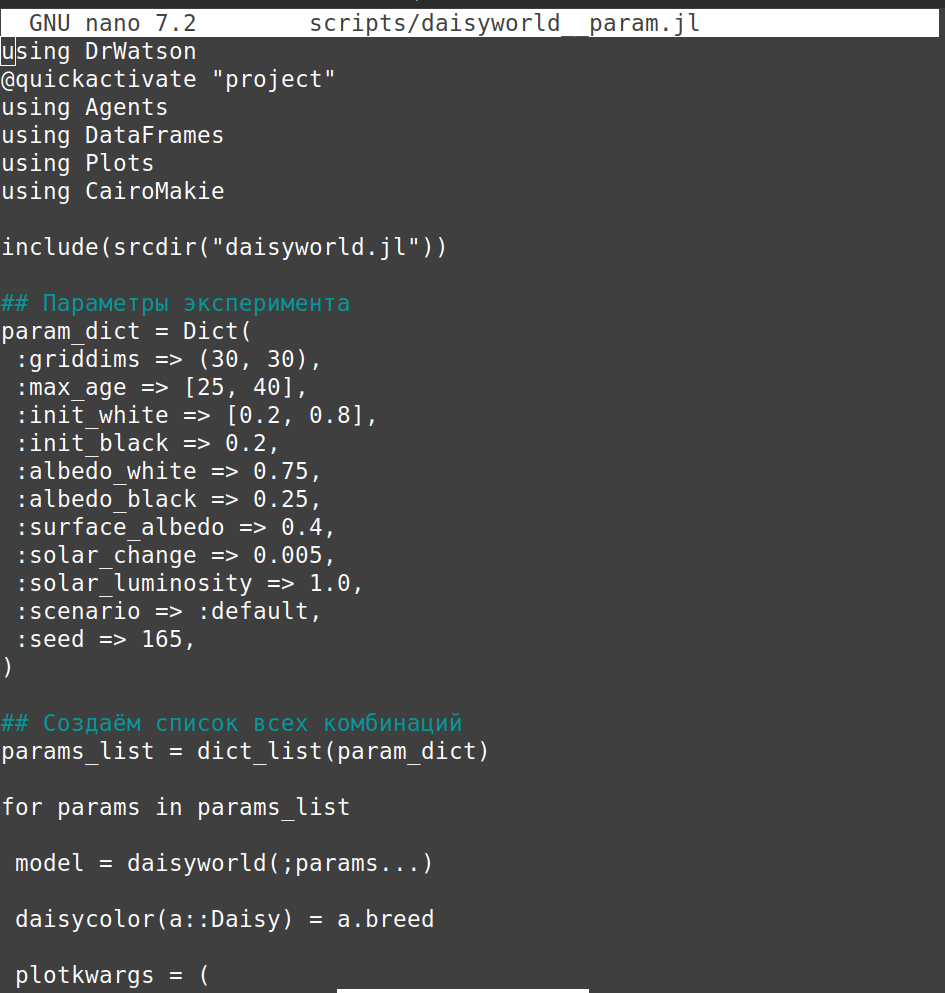
\includegraphics[width=0.7\textwidth,height=\textheight]{image/pic23.png}

}

\caption{\label{fig-017}запуск код}

\end{figure}%

\emph{Запустив моделирование с различными комбинациями максимального
возраста и начального процента белых маргариток, мы можем увидеть, как
эти параметры влияют на систему. Чем дольше живут маргаритки
(\texttt{max\_age\ =\ 40}), тем стабильнее и медленнее меняются узоры на
сетке. Черные и белые ромашки остаются на месте дольше. Когда срок
службы маргариток сокращается (\texttt{max\_age\ =\ 25}), узоры
становятся более динамичными, маргаритки постоянно отмирают и их
заменяют. Начальный процент также имеет значение на ранней стадии, если
мы начнем с преимущественно белых маргариток
(\texttt{init\_white\ =\ 0,8}), планета станет прохладнее; если мы
начнем с преимущественно черных ромашек (\texttt{init\_white\ =\ 0.2}),
то получится теплее. Но вот что интересно: независимо от того, какие
параметры мы используем, к тому времени, когда мы дойдем до 40 шагов,
все симуляции достигнут одинакового равновесия. Черные и белые
маргаритки располагаются чередующимися участками, а температура остается
в пределах допустимой для жизни.}

Запустив файл и посмотрев на результаты, я преобразовала его в
литературный стиль(рис.~\ref{fig-018})

\begin{figure}

\centering{


\includegraphics[width=0.7\textwidth,height=\textheight]{image/pic24.png}

}

\caption{\label{fig-018}преобразования кода в литературный}

\end{figure}%

Я генерирую следующие файлы из литературного кода: чистый код, jupyter
notebook и документация в формате Quarto. После этого я проверяю, чтобы
убедиться, что все ячейки в файле jupyter notebook работают без
ошибок(рис.~\ref{fig-019})

\begin{figure}

\centering{


\includegraphics[width=0.7\textwidth,height=\textheight]{image/pic25.png}

}

\caption{\label{fig-019}проверка работы код}

\end{figure}%

***Ниже приведен код, результаты расчетов и графики для кода в файле
scripts/daisyworld\_\_param.jl.qmd***

\chapter{Параметрическое исследование модели
Daisyworld}\label{ux43fux430ux440ux430ux43cux435ux442ux440ux438ux447ux435ux441ux43aux43eux435-ux438ux441ux441ux43bux435ux434ux43eux432ux430ux43dux438ux435-ux43cux43eux434ux435ux43bux438-daisyworld}

\section{Описание}\label{ux43eux43fux438ux441ux430ux43dux438ux435-3}

Этот скрипт проводит параметрическое исследование модели Daisyworld,
изучая влияние различных параметров на поведение системы. Для каждой
комбинации параметров генерируются три визуализации: - начальное
состояние (t = 0) - после 5 шагов моделирования - после 40 шагов
моделирования

Исследуемые параметры: - \texttt{max\_age} - максимальный возраст
маргариток (25 и 40 шагов) - \texttt{init\_white} - начальная доля белых
маргариток (20\% и 80\%)

\section{Подготовка
окружения}\label{ux43fux43eux434ux433ux43eux442ux43eux432ux43aux430-ux43eux43aux440ux443ux436ux435ux43dux438ux44f-3}

Активируем проект DrWatson и загружаем необходимые пакеты:

\begin{Shaded}
\begin{Highlighting}[]
\ImportTok{using} \BuiltInTok{DrWatson}
\PreprocessorTok{@quickactivate} \StringTok{"project"}

\ImportTok{using} \BuiltInTok{Agents}      \CommentTok{\# для агентного моделирования}
\ImportTok{using} \BuiltInTok{DataFrames}  \CommentTok{\# для работы с данными}
\ImportTok{using} \BuiltInTok{Plots}       \CommentTok{\# для визуализации}
\ImportTok{using} \BuiltInTok{CairoMakie}  \CommentTok{\# для высококачественной графики}
\end{Highlighting}
\end{Shaded}

\begin{verbatim}
┌ Warning: DrWatson could not find find a project file by recursively checking given `dir` and its parents. Returning `nothing` instead.
│ (given dir: /home/nelianjovu)
└ @ DrWatson ~/.julia/packages/DrWatson/2QF5p/src/project_setup.jl:84
\end{verbatim}

\section{Подключение
модели}\label{ux43fux43eux434ux43aux43bux44eux447ux435ux43dux438ux435-ux43cux43eux434ux435ux43bux438-3}

Подключаем файл с реализацией модели Daisyworld

\begin{Shaded}
\begin{Highlighting}[]
\FunctionTok{include}\NormalTok{(}\FunctionTok{srcdir}\NormalTok{(}\StringTok{"daisyworld.jl"}\NormalTok{))}
\end{Highlighting}
\end{Shaded}

\begin{verbatim}
daisyworld (generic function with 1 method)
\end{verbatim}

\section{Определение параметров
эксперимента}\label{ux43eux43fux440ux435ux434ux435ux43bux435ux43dux438ux435-ux43fux430ux440ux430ux43cux435ux442ux440ux43eux432-ux44dux43aux441ux43fux435ux440ux438ux43cux435ux43dux442ux430}

Задаём словарь с параметрами для исследования. Значения в векторах будут
комбинироваться для создания всех возможных сочетаний.

\begin{Shaded}
\begin{Highlighting}[]
\NormalTok{param\_dict }\OperatorTok{=} \FunctionTok{Dict}\NormalTok{(}\CommentTok{\# Фиксированные параметры}
    \OperatorTok{:}\NormalTok{griddims }\OperatorTok{=\textgreater{}}\NormalTok{ (}\FloatTok{30}\NormalTok{, }\FloatTok{30}\NormalTok{),           }\CommentTok{\# размер сетки 30×30}
    \OperatorTok{:}\NormalTok{init\_black }\OperatorTok{=\textgreater{}} \FloatTok{0.2}\NormalTok{,               }\CommentTok{\# начальная доля чёрных маргариток (20\%)}
    \OperatorTok{:}\NormalTok{albedo\_white }\OperatorTok{=\textgreater{}} \FloatTok{0.75}\NormalTok{,             }\CommentTok{\# альбедо белых маргариток}
    \OperatorTok{:}\NormalTok{albedo\_black }\OperatorTok{=\textgreater{}} \FloatTok{0.25}\NormalTok{,             }\CommentTok{\# альбедо чёрных маргариток}
    \OperatorTok{:}\NormalTok{surface\_albedo }\OperatorTok{=\textgreater{}} \FloatTok{0.4}\NormalTok{,            }\CommentTok{\# альбедо пустой поверхности}
    \OperatorTok{:}\NormalTok{solar\_change }\OperatorTok{=\textgreater{}} \FloatTok{0.005}\NormalTok{,            }\CommentTok{\# скорость изменения светимости}
    \OperatorTok{:}\NormalTok{solar\_luminosity }\OperatorTok{=\textgreater{}} \FloatTok{1.0}\NormalTok{,          }\CommentTok{\# начальная светимость}
    \OperatorTok{:}\NormalTok{scenario }\OperatorTok{=\textgreater{}} \OperatorTok{:}\NormalTok{default,              }\CommentTok{\# сценарий (без изменения светимости)}
    \OperatorTok{:}\NormalTok{seed }\OperatorTok{=\textgreater{}} \FloatTok{165}\NormalTok{,                       }\CommentTok{\# зерно для генератора случайных чисел}
    \OperatorTok{:}\NormalTok{max\_age }\OperatorTok{=\textgreater{}}\NormalTok{ [}\FloatTok{25}\NormalTok{, }\FloatTok{40}\NormalTok{],               }\CommentTok{\# максимальный возраст (два значения)}
    \OperatorTok{:}\NormalTok{init\_white }\OperatorTok{=\textgreater{}}\NormalTok{ [}\FloatTok{0.2}\NormalTok{, }\FloatTok{0.8}\NormalTok{],           }\CommentTok{\# начальная доля белых (20\% и 80\%)}
\NormalTok{)}

\FunctionTok{println}\NormalTok{(}\StringTok{"Параметры эксперимента:"}\NormalTok{)}
\FunctionTok{println}\NormalTok{(}\StringTok{"   {-} Варьируемые параметры: max\_age = [25, 40], init\_white = [0.2, 0.8]"}\NormalTok{)}
\FunctionTok{println}\NormalTok{(}\StringTok{"   {-} Фиксированные параметры: сетка 30×30, альбедо чёрных = 0.25, альбедо белых = 0.75"}\NormalTok{)}
\end{Highlighting}
\end{Shaded}

\begin{verbatim}
Параметры эксперимента:
   - Варьируемые параметры: max_age = [25, 40], init_white = [0.2, 0.8]
   - Фиксированные параметры: сетка 30×30, альбедо чёрных = 0.25, альбедо белых = 0.75
\end{verbatim}

\section{Генерация комбинаций
параметров}\label{ux433ux435ux43dux435ux440ux430ux446ux438ux44f-ux43aux43eux43cux431ux438ux43dux430ux446ux438ux439-ux43fux430ux440ux430ux43cux435ux442ux440ux43eux432}

Создаём список всех возможных комбинаций значений параметров с помощью
функции \texttt{dict\_list} из пакета DrWatson.

\begin{Shaded}
\begin{Highlighting}[]
\NormalTok{params\_list }\OperatorTok{=} \FunctionTok{dict\_list}\NormalTok{(param\_dict)}
\FunctionTok{println}\NormalTok{(}\StringTok{"Всего комбинаций параметров: "}\NormalTok{, }\FunctionTok{length}\NormalTok{(params\_list))}
\end{Highlighting}
\end{Shaded}

\begin{verbatim}
Всего комбинаций параметров: 4
\end{verbatim}

\section{Функция для цвета
агентов}\label{ux444ux443ux43dux43aux446ux438ux44f-ux434ux43bux44f-ux446ux432ux435ux442ux430-ux430ux433ux435ux43dux442ux43eux432}

Определяем функцию, которая возвращает цвет маргаритки в зависимости от
её типа:

\begin{Shaded}
\begin{Highlighting}[]
\FunctionTok{daisycolor}\NormalTok{(a}\OperatorTok{::}\DataTypeTok{Daisy}\NormalTok{) }\OperatorTok{=}\NormalTok{ a.breed  }\CommentTok{\# :black или :white}
\end{Highlighting}
\end{Shaded}

\begin{verbatim}
daisycolor (generic function with 1 method)
\end{verbatim}

\section{Настройка
визуализации}\label{ux43dux430ux441ux442ux440ux43eux439ux43aux430-ux432ux438ux437ux443ux430ux43bux438ux437ux430ux446ux438ux438-1}

Задаём общие параметры для всех графиков:

\begin{Shaded}
\begin{Highlighting}[]
\NormalTok{plotkwargs }\OperatorTok{=}\NormalTok{ (}
\NormalTok{    agent\_color }\OperatorTok{=}\NormalTok{ daisycolor,          }\CommentTok{\# цвет агентов (чёрный/белый)}
\NormalTok{    agent\_size }\OperatorTok{=} \FloatTok{20}\NormalTok{,                    }\CommentTok{\# размер маркеров}
\NormalTok{    agent\_marker }\OperatorTok{=} \CharTok{\textquotesingle{}✿\textquotesingle{}}\NormalTok{,                  }\CommentTok{\# символ для маргариток (цветок)}
\NormalTok{    heatarray }\OperatorTok{=} \OperatorTok{:}\NormalTok{temperature,            }\CommentTok{\# данные для тепловой карты}
\NormalTok{    heatkwargs }\OperatorTok{=}\NormalTok{ (colorrange }\OperatorTok{=}\NormalTok{ (}\OperatorTok{{-}}\FloatTok{20}\NormalTok{, }\FloatTok{60}\NormalTok{),),  }\CommentTok{\# диапазон температур}
\NormalTok{)}
\end{Highlighting}
\end{Shaded}

\begin{verbatim}
(agent_color = daisycolor, agent_size = 20, agent_marker = '✿', heatarray = :temperature, heatkwargs = (colorrange = (-20, 60),))
\end{verbatim}

\section{Цикл по всем комбинациям
параметров}\label{ux446ux438ux43aux43b-ux43fux43e-ux432ux441ux435ux43c-ux43aux43eux43cux431ux438ux43dux430ux446ux438ux44fux43c-ux43fux430ux440ux430ux43cux435ux442ux440ux43eux432}

Для каждого набора параметров: 1. Создаём модель 2. Визуализируем
начальное состояние 3. Выполняем 5 шагов и визуализируем 4. Выполняем до
40 шагов и визуализируем 5. Сохраняем все три графика с именами,
содержащими значения параметров

\begin{Shaded}
\begin{Highlighting}[]
\FunctionTok{println}\NormalTok{(}\StringTok{"ЗАПУСК ПАРАМЕТРИЧЕСКОГО ИССЛЕДОВАНИЯ"}\NormalTok{)}

\ControlFlowTok{for}\NormalTok{ (i, params) }\KeywordTok{in} \FunctionTok{enumerate}\NormalTok{(params\_list)}
    \FunctionTok{println}\NormalTok{(}\StringTok{"}\SpecialCharTok{\textbackslash{}n}\StringTok{Эксперимент }\SpecialCharTok{$}\NormalTok{i}\StringTok{/}\SpecialCharTok{$}\NormalTok{(}\FunctionTok{length}\NormalTok{(params\_list))}\StringTok{"}\NormalTok{)}
    \FunctionTok{println}\NormalTok{(}\StringTok{"   Параметры: max\_age = }\SpecialCharTok{$}\NormalTok{(params[}\OperatorTok{:}\NormalTok{max\_age])}\StringTok{, init\_white = }\SpecialCharTok{$}\NormalTok{(params[}\OperatorTok{:}\NormalTok{init\_white])}\StringTok{"}\NormalTok{)}

\NormalTok{    model }\OperatorTok{=} \FunctionTok{daisyworld}\NormalTok{(; params}\OperatorTok{...}\NormalTok{)}\CommentTok{\# Создание модели с текущими параметрами}
    \FunctionTok{println}\NormalTok{(}\StringTok{"Модель создана"}\NormalTok{)}

    \FunctionTok{println}\NormalTok{(}\StringTok{"Визуализация t = 0..."}\NormalTok{) }\CommentTok{\# Визуализация начального состояния (t = 0)}
\NormalTok{    plt1, \_ }\OperatorTok{=} \FunctionTok{abmplot}\NormalTok{(model; plotkwargs}\OperatorTok{...}\NormalTok{)}
\NormalTok{    fig1 }\OperatorTok{=} \FunctionTok{Figure}\NormalTok{(size }\OperatorTok{=}\NormalTok{ (}\FloatTok{800}\NormalTok{, }\FloatTok{600}\NormalTok{))}
\NormalTok{    ax1 }\OperatorTok{=} \FunctionTok{Axis}\NormalTok{(fig1[}\FloatTok{1}\NormalTok{,}\FloatTok{1}\NormalTok{], title }\OperatorTok{=} \StringTok{"Начальное состояние (t=0)}\SpecialCharTok{\textbackslash{}n}\StringTok{max\_age=}\SpecialCharTok{$}\NormalTok{(params[}\OperatorTok{:}\NormalTok{max\_age])}\StringTok{, init\_white=}\SpecialCharTok{$}\NormalTok{(params[}\OperatorTok{:}\NormalTok{init\_white])}\StringTok{"}\NormalTok{)}
    \FunctionTok{display}\NormalTok{(plt1)}

    \FunctionTok{step!}\NormalTok{(model, }\FloatTok{5}\NormalTok{)}\CommentTok{\# Моделирование 5 шагов}
    \FunctionTok{println}\NormalTok{(}\StringTok{"Визуализация t = 5..."}\NormalTok{)}
\NormalTok{    plt2, \_ }\OperatorTok{=} \FunctionTok{abmplot}\NormalTok{(model; heatarray }\OperatorTok{=}\NormalTok{ model.temperature, plotkwargs}\OperatorTok{...}\NormalTok{)}
    \FunctionTok{display}\NormalTok{(plt2)}
    \FunctionTok{step!}\NormalTok{(model, }\FloatTok{35}\NormalTok{)  }\CommentTok{\# Моделирование до 40 шагов}
    \FunctionTok{println}\NormalTok{(}\StringTok{"Визуализация t = 40..."}\NormalTok{)}
\NormalTok{    plt3, \_ }\OperatorTok{=} \FunctionTok{abmplot}\NormalTok{(model; heatarray }\OperatorTok{=}\NormalTok{ model.temperature, plotkwargs}\OperatorTok{...}\NormalTok{)}
    \FunctionTok{display}\NormalTok{(plt3)}

\NormalTok{    plt1\_name }\OperatorTok{=} \FunctionTok{savename}\NormalTok{(}\StringTok{"daisyworld"}\NormalTok{, params) }\OperatorTok{*} \StringTok{"\_step01.png"} \CommentTok{\# Формирование имён файлов}
\NormalTok{    plt2\_name }\OperatorTok{=} \FunctionTok{savename}\NormalTok{(}\StringTok{"daisyworld"}\NormalTok{, params) }\OperatorTok{*} \StringTok{"\_step05.png"}
\NormalTok{    plt3\_name }\OperatorTok{=} \FunctionTok{savename}\NormalTok{(}\StringTok{"daisyworld"}\NormalTok{, params) }\OperatorTok{*} \StringTok{"\_step40.png"}

    \FunctionTok{save}\NormalTok{(}\FunctionTok{plotsdir}\NormalTok{(plt1\_name), plt1)}\CommentTok{\#Сохранение графиков}
    \FunctionTok{save}\NormalTok{(}\FunctionTok{plotsdir}\NormalTok{(plt2\_name), plt2)}
    \FunctionTok{save}\NormalTok{(}\FunctionTok{plotsdir}\NormalTok{(plt3\_name), plt3)}

    \FunctionTok{println}\NormalTok{(}\StringTok{"Графики сохранены:"}\NormalTok{)}
    \FunctionTok{println}\NormalTok{(}\StringTok{"      {-} }\SpecialCharTok{$}\NormalTok{(plt1\_name)}\StringTok{"}\NormalTok{)}
    \FunctionTok{println}\NormalTok{(}\StringTok{"      {-} }\SpecialCharTok{$}\NormalTok{(plt2\_name)}\StringTok{"}\NormalTok{)}
    \FunctionTok{println}\NormalTok{(}\StringTok{"      {-} }\SpecialCharTok{$}\NormalTok{(plt3\_name)}\StringTok{"}\NormalTok{)}
\ControlFlowTok{end}
\end{Highlighting}
\end{Shaded}

\begin{verbatim}
ЗАПУСК ПАРАМЕТРИЧЕСКОГО ИССЛЕДОВАНИЯ

Эксперимент 1/4
   Параметры: max_age = 25, init_white = 0.2
Модель создана
Визуализация t = 0...
Визуализация t = 5...
Визуализация t = 40...
Графики сохранены:
      - daisyworld_albedo_black=0.25_albedo_white=0.75_init_black=0.2_init_white=0.2_max_age=25_scenario=default_seed=165_solar_change=0.005_solar_luminosity=1.0_surface_albedo=0.4_step01.png
      - daisyworld_albedo_black=0.25_albedo_white=0.75_init_black=0.2_init_white=0.2_max_age=25_scenario=default_seed=165_solar_change=0.005_solar_luminosity=1.0_surface_albedo=0.4_step05.png
      - daisyworld_albedo_black=0.25_albedo_white=0.75_init_black=0.2_init_white=0.2_max_age=25_scenario=default_seed=165_solar_change=0.005_solar_luminosity=1.0_surface_albedo=0.4_step40.png

Эксперимент 2/4
   Параметры: max_age = 25, init_white = 0.8
Модель создана
Визуализация t = 0...
Визуализация t = 5...
Визуализация t = 40...
Графики сохранены:
      - daisyworld_albedo_black=0.25_albedo_white=0.75_init_black=0.2_init_white=0.8_max_age=25_scenario=default_seed=165_solar_change=0.005_solar_luminosity=1.0_surface_albedo=0.4_step01.png
      - daisyworld_albedo_black=0.25_albedo_white=0.75_init_black=0.2_init_white=0.8_max_age=25_scenario=default_seed=165_solar_change=0.005_solar_luminosity=1.0_surface_albedo=0.4_step05.png
      - daisyworld_albedo_black=0.25_albedo_white=0.75_init_black=0.2_init_white=0.8_max_age=25_scenario=default_seed=165_solar_change=0.005_solar_luminosity=1.0_surface_albedo=0.4_step40.png

Эксперимент 3/4
   Параметры: max_age = 40, init_white = 0.2
Модель создана
Визуализация t = 0...
Визуализация t = 5...
Визуализация t = 40...
Графики сохранены:
      - daisyworld_albedo_black=0.25_albedo_white=0.75_init_black=0.2_init_white=0.2_max_age=40_scenario=default_seed=165_solar_change=0.005_solar_luminosity=1.0_surface_albedo=0.4_step01.png
      - daisyworld_albedo_black=0.25_albedo_white=0.75_init_black=0.2_init_white=0.2_max_age=40_scenario=default_seed=165_solar_change=0.005_solar_luminosity=1.0_surface_albedo=0.4_step05.png
      - daisyworld_albedo_black=0.25_albedo_white=0.75_init_black=0.2_init_white=0.2_max_age=40_scenario=default_seed=165_solar_change=0.005_solar_luminosity=1.0_surface_albedo=0.4_step40.png

Эксперимент 4/4
   Параметры: max_age = 40, init_white = 0.8
Модель создана
Визуализация t = 0...
Визуализация t = 5...
Визуализация t = 40...
Графики сохранены:
      - daisyworld_albedo_black=0.25_albedo_white=0.75_init_black=0.2_init_white=0.8_max_age=40_scenario=default_seed=165_solar_change=0.005_solar_luminosity=1.0_surface_albedo=0.4_step01.png
      - daisyworld_albedo_black=0.25_albedo_white=0.75_init_black=0.2_init_white=0.8_max_age=40_scenario=default_seed=165_solar_change=0.005_solar_luminosity=1.0_surface_albedo=0.4_step05.png
      - daisyworld_albedo_black=0.25_albedo_white=0.75_init_black=0.2_init_white=0.8_max_age=40_scenario=default_seed=165_solar_change=0.005_solar_luminosity=1.0_surface_albedo=0.4_step40.png
\end{verbatim}

\begin{verbatim}
┌ Warning: Found `resolution` in the theme when creating a `Scene`. The `resolution` keyword for `Scene`s and `Figure`s has been deprecated. Use `Figure(; size = ...` or `Scene(; size = ...)` instead, which better reflects that this is a unitless size and not a pixel resolution. The key could also come from `set_theme!` calls or related theming functions.
└ @ Makie ~/.julia/packages/Makie/kJl0u/src/scenes.jl:264
┌ Warning: Found `resolution` in the theme when creating a `Scene`. The `resolution` keyword for `Scene`s and `Figure`s has been deprecated. Use `Figure(; size = ...` or `Scene(; size = ...)` instead, which better reflects that this is a unitless size and not a pixel resolution. The key could also come from `set_theme!` calls or related theming functions.
└ @ Makie ~/.julia/packages/Makie/kJl0u/src/scenes.jl:264
┌ Warning: Found `resolution` in the theme when creating a `Scene`. The `resolution` keyword for `Scene`s and `Figure`s has been deprecated. Use `Figure(; size = ...` or `Scene(; size = ...)` instead, which better reflects that this is a unitless size and not a pixel resolution. The key could also come from `set_theme!` calls or related theming functions.
└ @ Makie ~/.julia/packages/Makie/kJl0u/src/scenes.jl:264
┌ Warning: Found `resolution` in the theme when creating a `Scene`. The `resolution` keyword for `Scene`s and `Figure`s has been deprecated. Use `Figure(; size = ...` or `Scene(; size = ...)` instead, which better reflects that this is a unitless size and not a pixel resolution. The key could also come from `set_theme!` calls or related theming functions.
└ @ Makie ~/.julia/packages/Makie/kJl0u/src/scenes.jl:264
┌ Warning: Found `resolution` in the theme when creating a `Scene`. The `resolution` keyword for `Scene`s and `Figure`s has been deprecated. Use `Figure(; size = ...` or `Scene(; size = ...)` instead, which better reflects that this is a unitless size and not a pixel resolution. The key could also come from `set_theme!` calls or related theming functions.
└ @ Makie ~/.julia/packages/Makie/kJl0u/src/scenes.jl:264
┌ Warning: Found `resolution` in the theme when creating a `Scene`. The `resolution` keyword for `Scene`s and `Figure`s has been deprecated. Use `Figure(; size = ...` or `Scene(; size = ...)` instead, which better reflects that this is a unitless size and not a pixel resolution. The key could also come from `set_theme!` calls or related theming functions.
└ @ Makie ~/.julia/packages/Makie/kJl0u/src/scenes.jl:264
┌ Warning: Found `resolution` in the theme when creating a `Scene`. The `resolution` keyword for `Scene`s and `Figure`s has been deprecated. Use `Figure(; size = ...` or `Scene(; size = ...)` instead, which better reflects that this is a unitless size and not a pixel resolution. The key could also come from `set_theme!` calls or related theming functions.
└ @ Makie ~/.julia/packages/Makie/kJl0u/src/scenes.jl:264
┌ Warning: Found `resolution` in the theme when creating a `Scene`. The `resolution` keyword for `Scene`s and `Figure`s has been deprecated. Use `Figure(; size = ...` or `Scene(; size = ...)` instead, which better reflects that this is a unitless size and not a pixel resolution. The key could also come from `set_theme!` calls or related theming functions.
└ @ Makie ~/.julia/packages/Makie/kJl0u/src/scenes.jl:264
┌ Warning: Found `resolution` in the theme when creating a `Scene`. The `resolution` keyword for `Scene`s and `Figure`s has been deprecated. Use `Figure(; size = ...` or `Scene(; size = ...)` instead, which better reflects that this is a unitless size and not a pixel resolution. The key could also come from `set_theme!` calls or related theming functions.
└ @ Makie ~/.julia/packages/Makie/kJl0u/src/scenes.jl:264
┌ Warning: Found `resolution` in the theme when creating a `Scene`. The `resolution` keyword for `Scene`s and `Figure`s has been deprecated. Use `Figure(; size = ...` or `Scene(; size = ...)` instead, which better reflects that this is a unitless size and not a pixel resolution. The key could also come from `set_theme!` calls or related theming functions.
└ @ Makie ~/.julia/packages/Makie/kJl0u/src/scenes.jl:264
┌ Warning: Found `resolution` in the theme when creating a `Scene`. The `resolution` keyword for `Scene`s and `Figure`s has been deprecated. Use `Figure(; size = ...` or `Scene(; size = ...)` instead, which better reflects that this is a unitless size and not a pixel resolution. The key could also come from `set_theme!` calls or related theming functions.
└ @ Makie ~/.julia/packages/Makie/kJl0u/src/scenes.jl:264
┌ Warning: Found `resolution` in the theme when creating a `Scene`. The `resolution` keyword for `Scene`s and `Figure`s has been deprecated. Use `Figure(; size = ...` or `Scene(; size = ...)` instead, which better reflects that this is a unitless size and not a pixel resolution. The key could also come from `set_theme!` calls or related theming functions.
└ @ Makie ~/.julia/packages/Makie/kJl0u/src/scenes.jl:264
┌ Warning: Found `resolution` in the theme when creating a `Scene`. The `resolution` keyword for `Scene`s and `Figure`s has been deprecated. Use `Figure(; size = ...` or `Scene(; size = ...)` instead, which better reflects that this is a unitless size and not a pixel resolution. The key could also come from `set_theme!` calls or related theming functions.
└ @ Makie ~/.julia/packages/Makie/kJl0u/src/scenes.jl:264
┌ Warning: Found `resolution` in the theme when creating a `Scene`. The `resolution` keyword for `Scene`s and `Figure`s has been deprecated. Use `Figure(; size = ...` or `Scene(; size = ...)` instead, which better reflects that this is a unitless size and not a pixel resolution. The key could also come from `set_theme!` calls or related theming functions.
└ @ Makie ~/.julia/packages/Makie/kJl0u/src/scenes.jl:264
┌ Warning: Found `resolution` in the theme when creating a `Scene`. The `resolution` keyword for `Scene`s and `Figure`s has been deprecated. Use `Figure(; size = ...` or `Scene(; size = ...)` instead, which better reflects that this is a unitless size and not a pixel resolution. The key could also come from `set_theme!` calls or related theming functions.
└ @ Makie ~/.julia/packages/Makie/kJl0u/src/scenes.jl:264
┌ Warning: Found `resolution` in the theme when creating a `Scene`. The `resolution` keyword for `Scene`s and `Figure`s has been deprecated. Use `Figure(; size = ...` or `Scene(; size = ...)` instead, which better reflects that this is a unitless size and not a pixel resolution. The key could also come from `set_theme!` calls or related theming functions.
└ @ Makie ~/.julia/packages/Makie/kJl0u/src/scenes.jl:264
\end{verbatim}


\includegraphics{simmod-lab03-report (Нджову Нелиа)_files/figure-pdf/cell-47-output-3.png}


\includegraphics{simmod-lab03-report (Нджову Нелиа)_files/figure-pdf/cell-47-output-4.png}


\includegraphics{simmod-lab03-report (Нджову Нелиа)_files/figure-pdf/cell-47-output-5.png}


\includegraphics{simmod-lab03-report (Нджову Нелиа)_files/figure-pdf/cell-47-output-6.png}


\includegraphics{simmod-lab03-report (Нджову Нелиа)_files/figure-pdf/cell-47-output-7.png}


\includegraphics{simmod-lab03-report (Нджову Нелиа)_files/figure-pdf/cell-47-output-8.png}


\includegraphics{simmod-lab03-report (Нджову Нелиа)_files/figure-pdf/cell-47-output-9.png}


\includegraphics{simmod-lab03-report (Нджову Нелиа)_files/figure-pdf/cell-47-output-10.png}


\includegraphics{simmod-lab03-report (Нджову Нелиа)_files/figure-pdf/cell-47-output-11.png}


\includegraphics{simmod-lab03-report (Нджову Нелиа)_files/figure-pdf/cell-47-output-12.png}


\includegraphics{simmod-lab03-report (Нджову Нелиа)_files/figure-pdf/cell-47-output-13.png}

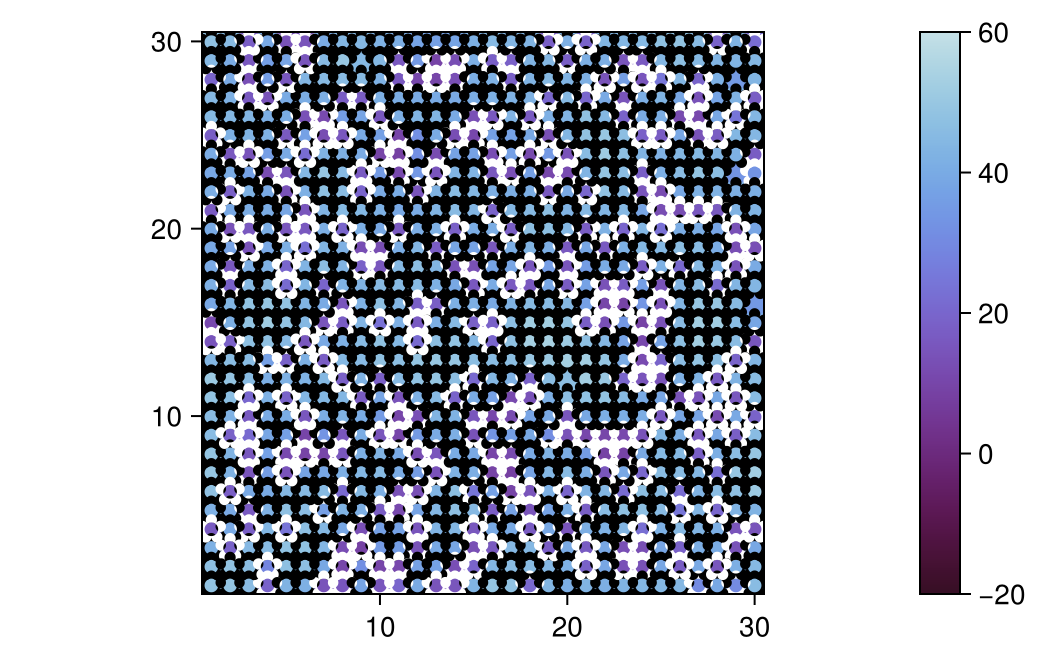
\includegraphics{simmod-lab03-report (Нджову Нелиа)_files/figure-pdf/cell-47-output-14.png}

\section{Итоги
эксперимента}\label{ux438ux442ux43eux433ux438-ux44dux43aux441ux43fux435ux440ux438ux43cux435ux43dux442ux430}

\begin{Shaded}
\begin{Highlighting}[]
\FunctionTok{println}\NormalTok{(}\StringTok{"ИТОГИ ПАРАМЕТРИЧЕСКОГО ИССЛЕДОВАНИЯ"}\NormalTok{)}
\FunctionTok{println}\NormalTok{(}\StringTok{"Всего выполнено экспериментов: "}\NormalTok{, }\FunctionTok{length}\NormalTok{(params\_list))}
\FunctionTok{println}\NormalTok{(}\StringTok{"Всего создано графиков: "}\NormalTok{, }\FunctionTok{length}\NormalTok{(params\_list) }\OperatorTok{*} \FloatTok{3}\NormalTok{)}
\FunctionTok{println}\NormalTok{(}\StringTok{"Графики сохранены в каталоге: "}\NormalTok{, }\FunctionTok{plotsdir}\NormalTok{())}
\end{Highlighting}
\end{Shaded}

\begin{verbatim}
ИТОГИ ПАРАМЕТРИЧЕСКОГО ИССЛЕДОВАНИЯ
Всего выполнено экспериментов: 4
Всего создано графиков: 12
Графики сохранены в каталоге: /home/nelianjovu/work/study/2026-1/2026-1==study--simulationmod/2026-1--study--simulationmod/labs/lab03/project/plots
\end{verbatim}

\section{7. Динамика числа
маргариток(параметры)}\label{ux434ux438ux43dux430ux43cux438ux43aux430-ux447ux438ux441ux43bux430-ux43cux430ux440ux433ux430ux440ux438ux442ux43eux43aux43fux430ux440ux430ux43cux435ux442ux440ux44b}

Я создала файл scripts/daisyworld-count\_\_param.jl и скопировала скрипт
код, который мне дали и запускала его. Этот скрипт выполняет
параметрическое исследование динамики популяции он запускает
моделирование Daisyworld в течение 1000 шагов с различными комбинациями
параметров и сохраняет графики популяции для каждого из
них(рис.~\ref{fig-020})

\begin{figure}

\centering{


\includegraphics[width=0.7\textwidth,height=\textheight]{image/pic26.png}

}

\caption{\label{fig-020}запуск код}

\end{figure}%

\emph{Рассматривая четыре графика рядом, мы можем видеть, как
максимальный возраст и начальные условия влияют на популяционные циклы.
Когда маргаритки живут дольше (\enquote{максимальный возраст = 40}),
подъемы и спады происходят медленнее и плавнее линии на графике
становятся шире и более изящными. Когда продолжительность жизни
маргариток сокращается (\texttt{max\_age\ =\ 25}), колебания становятся
более быстрыми и неустойчивыми, а популяции быстрее меняют направление.
Начальный процент в основном влияет на начало графика, если мы начинаем
с большего количества белых ромашек (\texttt{init\_white\ =\ 0.8}),
белая линия начинается выше, а черная ниже, и наоборот. После нескольких
сотен шагов все четыре графика начинают выглядеть довольно похоже. Все
они следуют одному и тому же ритму, в котором черные и белые ромашки по
очереди становятся все более многочисленными}

Запустив файл и посмотрев на результаты, я преобразовала его в
литературный стиль(рис.~\ref{fig-021})

\begin{figure}

\centering{

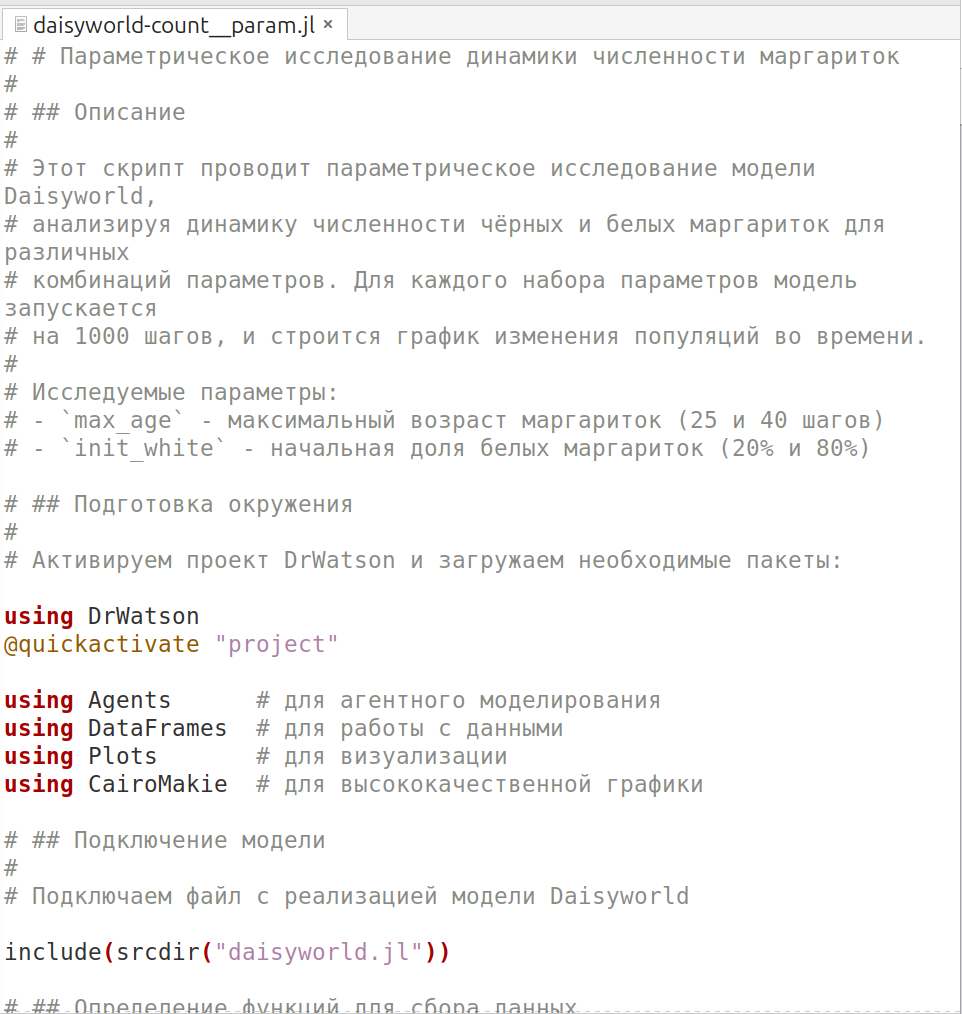
\includegraphics[width=0.7\textwidth,height=\textheight]{image/pic27.png}

}

\caption{\label{fig-021}преобразования кода в литературный}

\end{figure}%

Я генерирую следующие файлы из литературного кода: чистый код, jupyter
notebook и документация в формате Quarto. После этого я проверяю, чтобы
убедиться, что все ячейки в файле jupyter notebook работают без
ошибок(рис.~\ref{fig-022})

\begin{figure}

\centering{

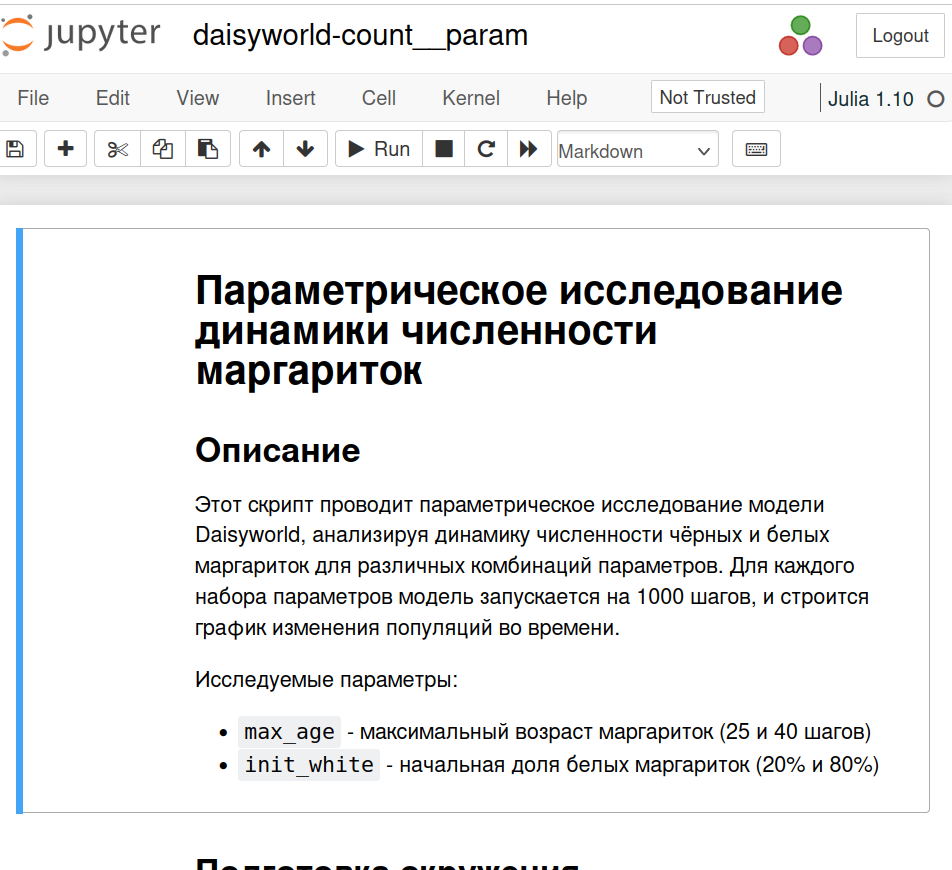
\includegraphics[width=0.7\textwidth,height=\textheight]{image/pic28.png}

}

\caption{\label{fig-022}проверка работы код}

\end{figure}%

***Ниже приведен код, результаты расчетов и графики для кода в файле
scripts/daisyworld-count\_\_param.jl.qmd***

\chapter{Параметрическое исследование динамики численности
маргариток}\label{ux43fux430ux440ux430ux43cux435ux442ux440ux438ux447ux435ux441ux43aux43eux435-ux438ux441ux441ux43bux435ux434ux43eux432ux430ux43dux438ux435-ux434ux438ux43dux430ux43cux438ux43aux438-ux447ux438ux441ux43bux435ux43dux43dux43eux441ux442ux438-ux43cux430ux440ux433ux430ux440ux438ux442ux43eux43a}

\section{Описание}\label{ux43eux43fux438ux441ux430ux43dux438ux435-4}

Этот скрипт проводит параметрическое исследование модели Daisyworld,
анализируя динамику численности чёрных и белых маргариток для различных
комбинаций параметров. Для каждого набора параметров модель запускается
на 1000 шагов, и строится график изменения популяций во времени.

Исследуемые параметры: - \texttt{max\_age} - максимальный возраст
маргариток (25 и 40 шагов) - \texttt{init\_white} - начальная доля белых
маргариток (20\% и 80\%)

\section{Подготовка
окружения}\label{ux43fux43eux434ux433ux43eux442ux43eux432ux43aux430-ux43eux43aux440ux443ux436ux435ux43dux438ux44f-4}

Активируем проект DrWatson и загружаем необходимые пакеты:

\begin{Shaded}
\begin{Highlighting}[]
\ImportTok{using} \BuiltInTok{DrWatson}
\PreprocessorTok{@quickactivate} \StringTok{"project"}

\ImportTok{using} \BuiltInTok{Agents}      \CommentTok{\# для агентного моделирования}
\ImportTok{using} \BuiltInTok{DataFrames}  \CommentTok{\# для работы с данными}
\ImportTok{using} \BuiltInTok{Plots}       \CommentTok{\# для визуализации}
\ImportTok{using} \BuiltInTok{CairoMakie}  \CommentTok{\# для высококачественной графики}
\end{Highlighting}
\end{Shaded}

\begin{verbatim}
┌ Warning: DrWatson could not find find a project file by recursively checking given `dir` and its parents. Returning `nothing` instead.
│ (given dir: /home/nelianjovu)
└ @ DrWatson ~/.julia/packages/DrWatson/2QF5p/src/project_setup.jl:84
\end{verbatim}

\section{Подключение
модели}\label{ux43fux43eux434ux43aux43bux44eux447ux435ux43dux438ux435-ux43cux43eux434ux435ux43bux438-4}

Подключаем файл с реализацией модели Daisyworld

\begin{Shaded}
\begin{Highlighting}[]
\FunctionTok{include}\NormalTok{(}\FunctionTok{srcdir}\NormalTok{(}\StringTok{"daisyworld.jl"}\NormalTok{))}
\end{Highlighting}
\end{Shaded}

\begin{verbatim}
daisyworld (generic function with 1 method)
\end{verbatim}

\section{Определение функций для сбора
данных}\label{ux43eux43fux440ux435ux434ux435ux43bux435ux43dux438ux435-ux444ux443ux43dux43aux446ux438ux439-ux434ux43bux44f-ux441ux431ux43eux440ux430-ux434ux430ux43dux43dux44bux445-2}

Создаём функции-предикаты для идентификации типа маргариток:

\begin{Shaded}
\begin{Highlighting}[]
\FunctionTok{black}\NormalTok{(a}\OperatorTok{::}\DataTypeTok{Daisy}\NormalTok{) }\OperatorTok{=}\NormalTok{ a.breed }\OperatorTok{==} \OperatorTok{:}\NormalTok{black}
\FunctionTok{white}\NormalTok{(a}\OperatorTok{::}\DataTypeTok{Daisy}\NormalTok{) }\OperatorTok{=}\NormalTok{ a.breed }\OperatorTok{==} \OperatorTok{:}\NormalTok{white}
\end{Highlighting}
\end{Shaded}

\begin{verbatim}
white (generic function with 1 method)
\end{verbatim}

\section{Настройка сбора
данных}\label{ux43dux430ux441ux442ux440ux43eux439ux43aux430-ux441ux431ux43eux440ux430-ux434ux430ux43dux43dux44bux445-2}

Указываем, какие данные собирать в процессе моделирования: - для чёрных
маргариток: подсчёт количества - для белых маргариток: подсчёт
количества

\begin{Shaded}
\begin{Highlighting}[]
\NormalTok{adata }\OperatorTok{=}\NormalTok{ [(black, count), (white, count)]}
\end{Highlighting}
\end{Shaded}

\begin{verbatim}
2-element Vector{Tuple{Function, typeof(count)}}:
 (black, count)
 (white, count)
\end{verbatim}

\section{Определение параметров
эксперимента}\label{ux43eux43fux440ux435ux434ux435ux43bux435ux43dux438ux435-ux43fux430ux440ux430ux43cux435ux442ux440ux43eux432-ux44dux43aux441ux43fux435ux440ux438ux43cux435ux43dux442ux430-1}

Задаём словарь с параметрами для исследования. Значения в векторах будут
комбинироваться для создания всех возможных сочетаний.

\begin{Shaded}
\begin{Highlighting}[]
\NormalTok{param\_dict }\OperatorTok{=} \FunctionTok{Dict}\NormalTok{(}\CommentTok{\# Фиксированные параметры}
    \OperatorTok{:}\NormalTok{griddims }\OperatorTok{=\textgreater{}}\NormalTok{ (}\FloatTok{30}\NormalTok{, }\FloatTok{30}\NormalTok{),           }\CommentTok{\# размер сетки 30×30}
    \OperatorTok{:}\NormalTok{init\_black }\OperatorTok{=\textgreater{}} \FloatTok{0.2}\NormalTok{,               }\CommentTok{\# начальная доля чёрных маргариток (20\%)}
    \OperatorTok{:}\NormalTok{albedo\_white }\OperatorTok{=\textgreater{}} \FloatTok{0.75}\NormalTok{,             }\CommentTok{\# альбедо белых маргариток}
    \OperatorTok{:}\NormalTok{albedo\_black }\OperatorTok{=\textgreater{}} \FloatTok{0.25}\NormalTok{,             }\CommentTok{\# альбедо чёрных маргариток}
    \OperatorTok{:}\NormalTok{surface\_albedo }\OperatorTok{=\textgreater{}} \FloatTok{0.4}\NormalTok{,            }\CommentTok{\# альбедо пустой поверхности}
    \OperatorTok{:}\NormalTok{solar\_change }\OperatorTok{=\textgreater{}} \FloatTok{0.005}\NormalTok{,            }\CommentTok{\# скорость изменения светимости}
    \OperatorTok{:}\NormalTok{solar\_luminosity }\OperatorTok{=\textgreater{}} \FloatTok{1.0}\NormalTok{,          }\CommentTok{\# начальная светимость}
    \OperatorTok{:}\NormalTok{scenario }\OperatorTok{=\textgreater{}} \OperatorTok{:}\NormalTok{default,              }\CommentTok{\# сценарий (без изменения светимости)}
    \OperatorTok{:}\NormalTok{seed }\OperatorTok{=\textgreater{}} \FloatTok{165}\NormalTok{,                       }\CommentTok{\# зерно для генератора случайных чисел}
    \OperatorTok{:}\NormalTok{max\_age }\OperatorTok{=\textgreater{}}\NormalTok{ [}\FloatTok{25}\NormalTok{, }\FloatTok{40}\NormalTok{],               }\CommentTok{\# максимальный возраст (два значения)}
    \OperatorTok{:}\NormalTok{init\_white }\OperatorTok{=\textgreater{}}\NormalTok{ [}\FloatTok{0.2}\NormalTok{, }\FloatTok{0.8}\NormalTok{],           }\CommentTok{\# начальная доля белых (20\% и 80\%)}
\NormalTok{)}

\FunctionTok{println}\NormalTok{(}\StringTok{"Параметры эксперимента:"}\NormalTok{)}
\FunctionTok{println}\NormalTok{(}\StringTok{"   {-} Варьируемые параметры: max\_age ∈ [25, 40], init\_white ∈ [0.2, 0.8]"}\NormalTok{)}
\FunctionTok{println}\NormalTok{(}\StringTok{"   {-} Фиксированные параметры: сетка 30×30, init\_black = 0.2"}\NormalTok{)}
\FunctionTok{println}\NormalTok{(}\StringTok{"   {-} Всего комбинаций: }\SpecialCharTok{$}\NormalTok{(}\FunctionTok{length}\NormalTok{(param\_dict[}\OperatorTok{:}\NormalTok{max\_age]) }\OperatorTok{*} \FunctionTok{length}\NormalTok{(param\_dict[}\OperatorTok{:}\NormalTok{init\_white]))}\StringTok{"}\NormalTok{)}
\end{Highlighting}
\end{Shaded}

\begin{verbatim}
Параметры эксперимента:
   - Варьируемые параметры: max_age ∈ [25, 40], init_white ∈ [0.2, 0.8]
   - Фиксированные параметры: сетка 30×30, init_black = 0.2
   - Всего комбинаций: 4
\end{verbatim}

\section{Генерация комбинаций
параметров}\label{ux433ux435ux43dux435ux440ux430ux446ux438ux44f-ux43aux43eux43cux431ux438ux43dux430ux446ux438ux439-ux43fux430ux440ux430ux43cux435ux442ux440ux43eux432-1}

Создаём список всех возможных комбинаций значений параметров с помощью
функции \texttt{dict\_list} из пакета DrWatson.

\begin{Shaded}
\begin{Highlighting}[]
\NormalTok{params\_list }\OperatorTok{=} \FunctionTok{dict\_list}\NormalTok{(param\_dict)}
\FunctionTok{println}\NormalTok{(}\StringTok{"Сгенерировано комбинаций параметров: "}\NormalTok{, }\FunctionTok{length}\NormalTok{(params\_list))}
\end{Highlighting}
\end{Shaded}

\begin{verbatim}
Сгенерировано комбинаций параметров: 4
\end{verbatim}

\section{Цикл по всем комбинациям
параметров}\label{ux446ux438ux43aux43b-ux43fux43e-ux432ux441ux435ux43c-ux43aux43eux43cux431ux438ux43dux430ux446ux438ux44fux43c-ux43fux430ux440ux430ux43cux435ux442ux440ux43eux432-1}

Для каждого набора параметров: 1. Создаём модель 2. Запускаем
моделирование на 1000 шагов 3. Строим график динамики численности 4.
Сохраняем график с именем, содержащим значения параметров

\begin{Shaded}
\begin{Highlighting}[]
\FunctionTok{println}\NormalTok{(}\StringTok{"ЗАПУСК ПАРАМЕТРИЧЕСКОГО ИССЛЕДОВАНИЯ"}\NormalTok{)}

\ControlFlowTok{for}\NormalTok{ (i, params) }\KeywordTok{in} \FunctionTok{enumerate}\NormalTok{(params\_list)}
    \FunctionTok{println}\NormalTok{(}\StringTok{"}\SpecialCharTok{\textbackslash{}n}\StringTok{Эксперимент }\SpecialCharTok{$}\NormalTok{i}\StringTok{/}\SpecialCharTok{$}\NormalTok{(}\FunctionTok{length}\NormalTok{(params\_list))}\StringTok{"}\NormalTok{)}
    \FunctionTok{println}\NormalTok{(}\StringTok{"   Параметры: max\_age = }\SpecialCharTok{$}\NormalTok{(params[}\OperatorTok{:}\NormalTok{max\_age])}\StringTok{, init\_white = }\SpecialCharTok{$}\NormalTok{(params[}\OperatorTok{:}\NormalTok{init\_white])}\StringTok{"}\NormalTok{)}

\NormalTok{    model }\OperatorTok{=} \FunctionTok{daisyworld}\NormalTok{(; params}\OperatorTok{...}\NormalTok{)}\CommentTok{\# Создание модели с текущими параметрами}
    \FunctionTok{println}\NormalTok{(}\StringTok{"Модель создана"}\NormalTok{)}

    \FunctionTok{println}\NormalTok{(}\StringTok{"Запуск моделирования на 1000 шагов..."}\NormalTok{)}\CommentTok{\# Запуск моделирования. Выполняем 1000 шагов и собираем данные о популяциях.}
\NormalTok{    agent\_df, model\_df }\OperatorTok{=} \FunctionTok{run!}\NormalTok{(model, }\FloatTok{1000}\NormalTok{; adata)}
    \FunctionTok{println}\NormalTok{(}\StringTok{"Моделирование завершено"}\NormalTok{)}
    \FunctionTok{println}\NormalTok{(}\StringTok{"      {-} Собрано }\SpecialCharTok{$}\NormalTok{(}\FunctionTok{nrow}\NormalTok{(agent\_df))}\StringTok{ записей"}\NormalTok{)}
    \FunctionTok{println}\NormalTok{(}\StringTok{"      {-} Финальная численность: чёрные = }\SpecialCharTok{$}\NormalTok{(agent\_df.count\_black[}\KeywordTok{end}\NormalTok{])}\StringTok{, белые = }\SpecialCharTok{$}\NormalTok{(agent\_df.count\_white[}\KeywordTok{end}\NormalTok{])}\StringTok{"}\NormalTok{)}

\NormalTok{    figure }\OperatorTok{=} \FunctionTok{Figure}\NormalTok{(size }\OperatorTok{=}\NormalTok{ (}\FloatTok{600}\NormalTok{, }\FloatTok{400}\NormalTok{))}\CommentTok{\# Создание визуализации}

\NormalTok{    ax }\OperatorTok{=} \FunctionTok{Axis}\NormalTok{(figure[}\FloatTok{1}\NormalTok{, }\FloatTok{1}\NormalTok{], }\CommentTok{\# Создаём оси с подписями}
\NormalTok{              xlabel }\OperatorTok{=} \StringTok{"Время (шаги)"}\NormalTok{,}
\NormalTok{              ylabel }\OperatorTok{=} \StringTok{"Количество маргариток"}\NormalTok{,}
\NormalTok{              title }\OperatorTok{=} \StringTok{"Динамика численности (max\_age=}\SpecialCharTok{$}\NormalTok{(params[}\OperatorTok{:}\NormalTok{max\_age])}\StringTok{, init\_white=}\SpecialCharTok{$}\NormalTok{(params[}\OperatorTok{:}\NormalTok{init\_white])}\StringTok{)"}\NormalTok{)}\CommentTok{\# Создаём оси с подписями}

\NormalTok{    black\_line }\OperatorTok{=} \FunctionTok{lines!}\NormalTok{(ax, agent\_df[!, }\OperatorTok{:}\NormalTok{time],}
\NormalTok{                        color }\OperatorTok{=} \OperatorTok{:}\NormalTok{black, linewidth }\OperatorTok{=} \FloatTok{2}\NormalTok{, label }\OperatorTok{=} \StringTok{"Чёрные"}\NormalTok{)}
\NormalTok{    white\_line }\OperatorTok{=} \FunctionTok{lines!}\NormalTok{(ax, agent\_df[!, }\OperatorTok{:}\NormalTok{time], agent\_df[!, }\OperatorTok{:}\NormalTok{count\_white],}
\NormalTok{                        color }\OperatorTok{=} \OperatorTok{:}\NormalTok{orange, linewidth }\OperatorTok{=} \FloatTok{2}\NormalTok{, label }\OperatorTok{=} \StringTok{"Белые"}\NormalTok{)}\CommentTok{\# Строим линии для чёрных и белых маргариток agent\_df[!, :count\_black]}

    \FunctionTok{Legend}\NormalTok{(figure[}\FloatTok{1}\NormalTok{, }\FloatTok{2}\NormalTok{], [black\_line, white\_line], [}\StringTok{"Чёрные"}\NormalTok{, }\StringTok{"Белые"}\NormalTok{], labelsize }\OperatorTok{=} \FloatTok{12}\NormalTok{) }\CommentTok{\# Добавляем легенду}

    \FunctionTok{display}\NormalTok{(figure)}

\NormalTok{    plt\_name }\OperatorTok{=} \FunctionTok{savename}\NormalTok{(}\StringTok{"daisy{-}count"}\NormalTok{, params) }\OperatorTok{*} \StringTok{".png"}
    \FunctionTok{save}\NormalTok{(}\FunctionTok{plotsdir}\NormalTok{(plt\_name), figure)}\CommentTok{\# Сохранение графика}

    \FunctionTok{println}\NormalTok{(}\StringTok{"График сохранён: }\SpecialCharTok{$}\NormalTok{(plt\_name)}\StringTok{"}\NormalTok{)}
\ControlFlowTok{end}
\end{Highlighting}
\end{Shaded}

\begin{verbatim}
ЗАПУСК ПАРАМЕТРИЧЕСКОГО ИССЛЕДОВАНИЯ

Эксперимент 1/4
   Параметры: max_age = 25, init_white = 0.2
Модель создана
Запуск моделирования на 1000 шагов...
Моделирование завершено
      - Собрано 1001 записей
      - Финальная численность: чёрные = 669, белые = 231
График сохранён: daisy-count_albedo_black=0.25_albedo_white=0.75_init_black=0.2_init_white=0.2_max_age=25_scenario=default_seed=165_solar_change=0.005_solar_luminosity=1.0_surface_albedo=0.4.png

Эксперимент 2/4
   Параметры: max_age = 25, init_white = 0.8
Модель создана
Запуск моделирования на 1000 шагов...
Моделирование завершено
      - Собрано 1001 записей
      - Финальная численность: чёрные = 510, белые = 388
График сохранён: daisy-count_albedo_black=0.25_albedo_white=0.75_init_black=0.2_init_white=0.8_max_age=25_scenario=default_seed=165_solar_change=0.005_solar_luminosity=1.0_surface_albedo=0.4.png

Эксперимент 3/4
   Параметры: max_age = 40, init_white = 0.2
Модель создана
Запуск моделирования на 1000 шагов...
Моделирование завершено
      - Собрано 1001 записей
      - Финальная численность: чёрные = 502, белые = 392
График сохранён: daisy-count_albedo_black=0.25_albedo_white=0.75_init_black=0.2_init_white=0.2_max_age=40_scenario=default_seed=165_solar_change=0.005_solar_luminosity=1.0_surface_albedo=0.4.png

Эксперимент 4/4
   Параметры: max_age = 40, init_white = 0.8
Модель создана
Запуск моделирования на 1000 шагов...
Моделирование завершено
      - Собрано 1001 записей
      - Финальная численность: чёрные = 487, белые = 412
График сохранён: daisy-count_albedo_black=0.25_albedo_white=0.75_init_black=0.2_init_white=0.8_max_age=40_scenario=default_seed=165_solar_change=0.005_solar_luminosity=1.0_surface_albedo=0.4.png
\end{verbatim}

\begin{verbatim}
┌ Warning: Found `resolution` in the theme when creating a `Scene`. The `resolution` keyword for `Scene`s and `Figure`s has been deprecated. Use `Figure(; size = ...` or `Scene(; size = ...)` instead, which better reflects that this is a unitless size and not a pixel resolution. The key could also come from `set_theme!` calls or related theming functions.
└ @ Makie ~/.julia/packages/Makie/kJl0u/src/scenes.jl:264
┌ Warning: Found `resolution` in the theme when creating a `Scene`. The `resolution` keyword for `Scene`s and `Figure`s has been deprecated. Use `Figure(; size = ...` or `Scene(; size = ...)` instead, which better reflects that this is a unitless size and not a pixel resolution. The key could also come from `set_theme!` calls or related theming functions.
└ @ Makie ~/.julia/packages/Makie/kJl0u/src/scenes.jl:264
┌ Warning: Found `resolution` in the theme when creating a `Scene`. The `resolution` keyword for `Scene`s and `Figure`s has been deprecated. Use `Figure(; size = ...` or `Scene(; size = ...)` instead, which better reflects that this is a unitless size and not a pixel resolution. The key could also come from `set_theme!` calls or related theming functions.
└ @ Makie ~/.julia/packages/Makie/kJl0u/src/scenes.jl:264
┌ Warning: Found `resolution` in the theme when creating a `Scene`. The `resolution` keyword for `Scene`s and `Figure`s has been deprecated. Use `Figure(; size = ...` or `Scene(; size = ...)` instead, which better reflects that this is a unitless size and not a pixel resolution. The key could also come from `set_theme!` calls or related theming functions.
└ @ Makie ~/.julia/packages/Makie/kJl0u/src/scenes.jl:264
\end{verbatim}


\includegraphics{simmod-lab03-report (Нджову Нелиа)_files/figure-pdf/cell-55-output-3.png}


\includegraphics{simmod-lab03-report (Нджову Нелиа)_files/figure-pdf/cell-55-output-4.png}


\includegraphics{simmod-lab03-report (Нджову Нелиа)_files/figure-pdf/cell-55-output-5.png}

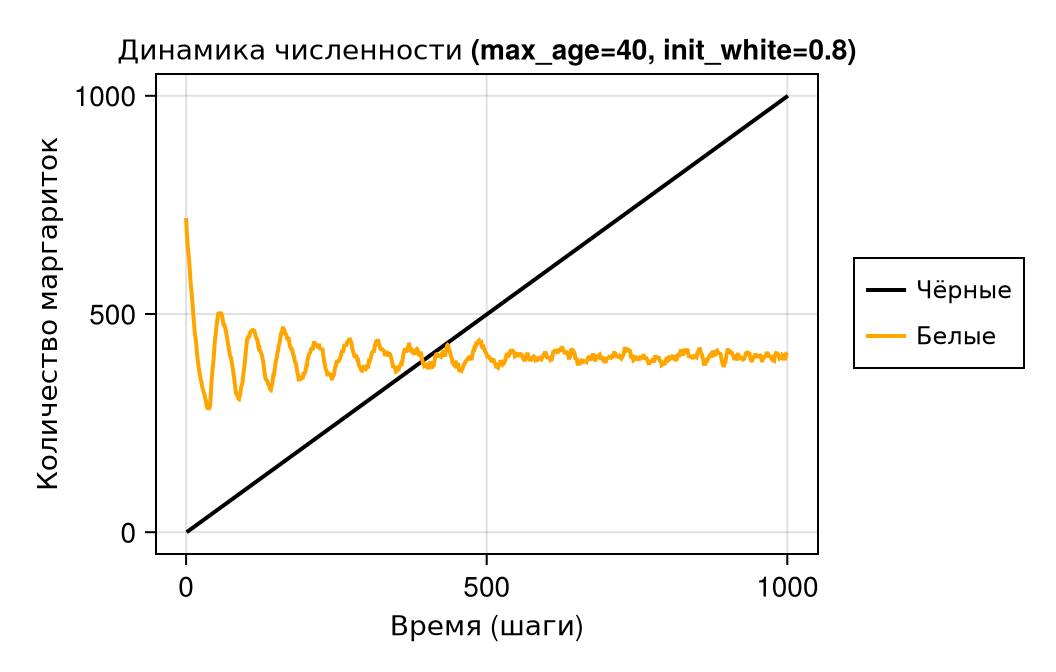
\includegraphics{simmod-lab03-report (Нджову Нелиа)_files/figure-pdf/cell-55-output-6.png}

\section{8. Динамика
модели(параметры)}\label{ux434ux438ux43dux430ux43cux438ux43aux430-ux43cux43eux434ux435ux43bux438ux43fux430ux440ux430ux43cux435ux442ux440ux44b}

Я создала файл scripts/daisyworld-luminosity\_\_param.jl и скопировала
скрипт код, который мне дали и запускала его. Этот скрипт выполняет
параметрическое исследование Daisyworld по сценарию :ramp он запускает
моделирование с различными комбинациями параметров, в то время как
яркость солнца увеличивается, а затем уменьшается:(рис.~\ref{fig-023})

\begin{figure}

\centering{

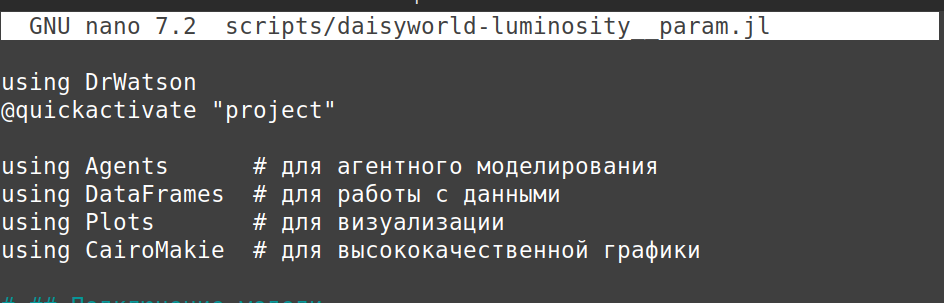
\includegraphics[width=0.7\textwidth,height=\textheight]{image/pic30.png}

}

\caption{\label{fig-023}запуск код}

\end{figure}%

\emph{Эти четыре графика показывают, что происходит, когда мы меняем
продолжительность жизни маргариток и количество цветов каждого вида, а
также время восхода и захода солнца. Нижняя панель на каждом графике
показывает яркость солнца, которая во всех экспериментах изменяется по
одной и той же схеме: она повышается, некоторое время остается высокой,
а затем снова снижается. Средняя панель показывает температуру, а
верхняя - численность маргариток. Что действительно здорово, так это то,
что независимо от того, какие параметры мы используем, температура
(средняя панель) всегда остается более стабильной, чем можно было бы
ожидать, учитывая, насколько сильно меняется температура на солнце.
Когда солнце становится ярче, белых маргариток (синяя линия) становится
больше, чтобы охладить обстановку; когда солнце становится тусклее,
черных маргариток (красная линия) становится больше, чтобы согреть
обстановку. Посмотрите на различия между графиками: когда маргаритки
живут дольше (\texttt{max\_age\ =\ 40}), температурная линия более
плавная, а изменения численности более постепенные; когда маргаритки
живут короче (\texttt{max\_age\ =\ 25}), все реагирует быстрее, а линии
более нервные. Начальный процент в основном влияет на начало, но через
некоторое время все графики начинают выглядеть одинаково. Это говорит
нам о том, что саморегуляция Daisyworld работает, несмотря ни на что}

Запустив файл и посмотрев на результаты, я преобразовала его в
литературный стиль(рис.~\ref{fig-024})

\begin{figure}

\centering{

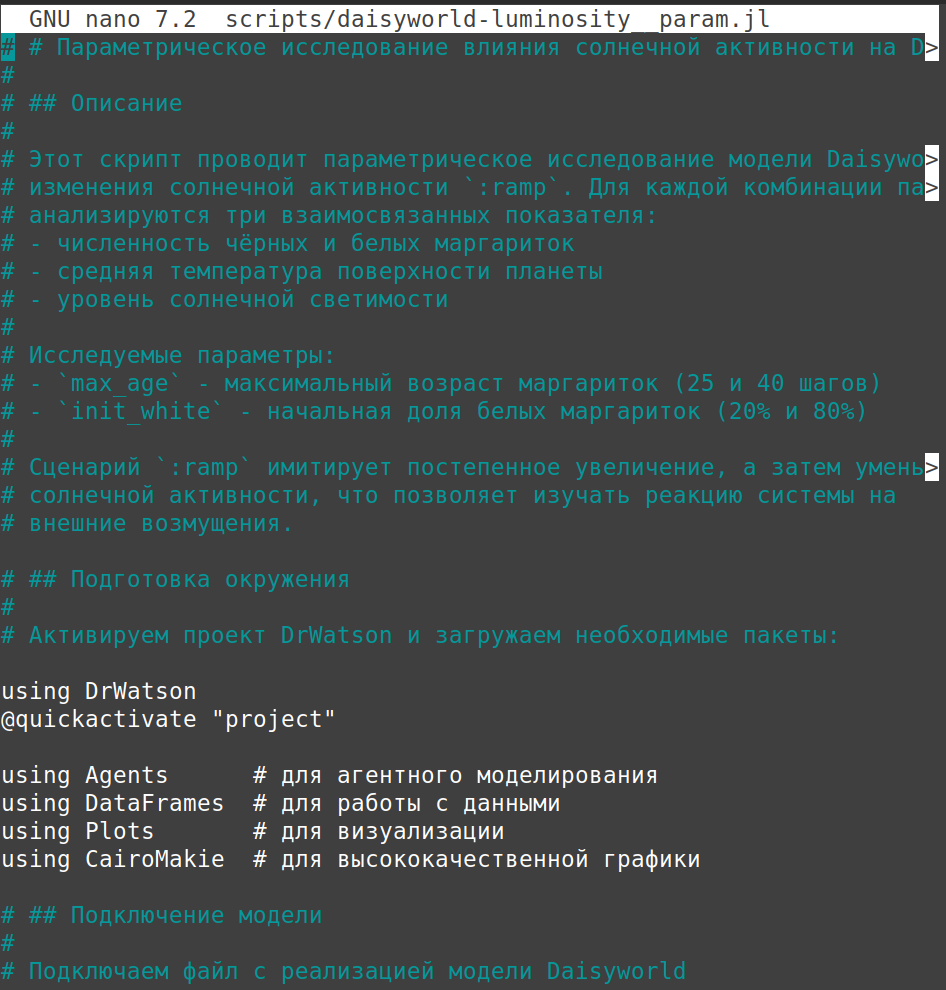
\includegraphics[width=0.7\textwidth,height=\textheight]{image/pic31.png}

}

\caption{\label{fig-024}преобразования кода в литературный}

\end{figure}%

Я генерирую следующие файлы из литературного кода: чистый код, jupyter
notebook и документация в формате Quarto. После этого я проверяю, чтобы
убедиться, что все ячейки в файле jupyter notebook работают без
ошибок(рис.~\ref{fig-025})

\begin{figure}

\centering{

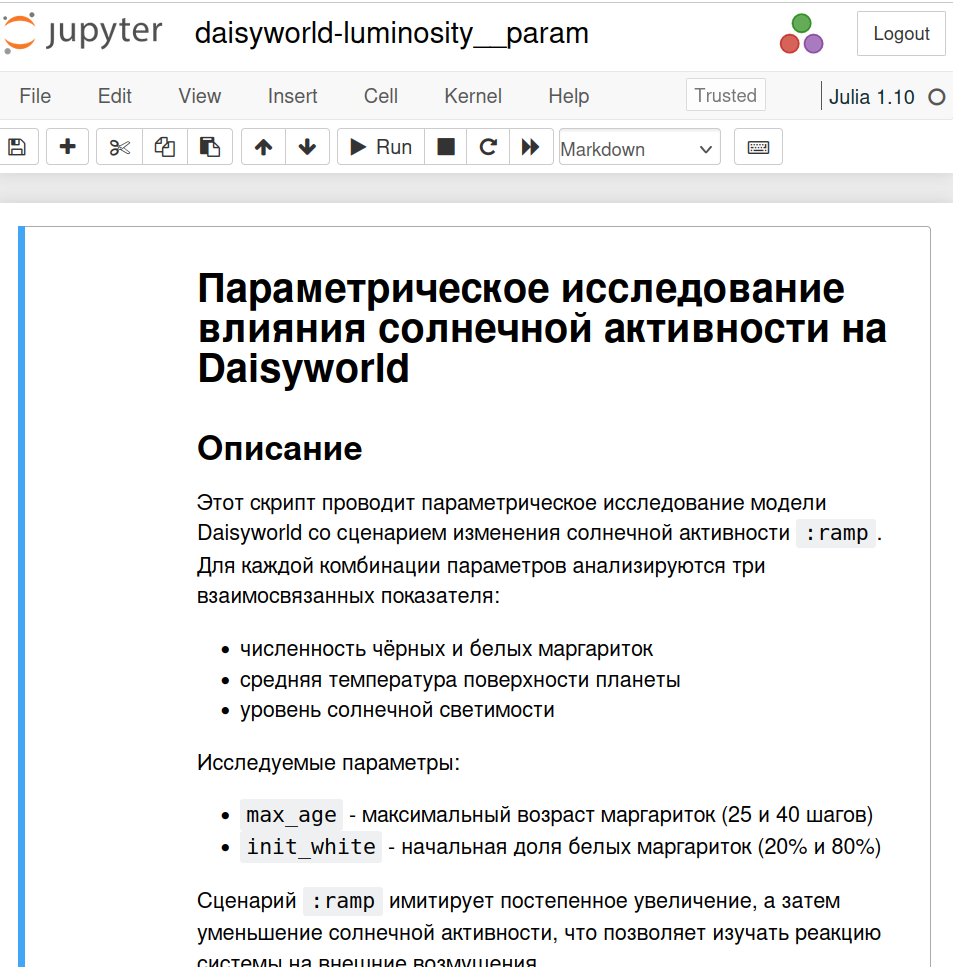
\includegraphics[width=0.7\textwidth,height=\textheight]{image/pic33.png}

}

\caption{\label{fig-025}проверка работы код}

\end{figure}%

***Ниже приведен код, результаты расчетов и графики для кода в файле
scripts/daisyworld-luminosity\_\_param.jl.qmd***

\chapter{Параметрическое исследование влияния солнечной активности на
Daisyworld}\label{ux43fux430ux440ux430ux43cux435ux442ux440ux438ux447ux435ux441ux43aux43eux435-ux438ux441ux441ux43bux435ux434ux43eux432ux430ux43dux438ux435-ux432ux43bux438ux44fux43dux438ux44f-ux441ux43eux43bux43dux435ux447ux43dux43eux439-ux430ux43aux442ux438ux432ux43dux43eux441ux442ux438-ux43dux430-daisyworld}

\section{Описание}\label{ux43eux43fux438ux441ux430ux43dux438ux435-5}

Этот скрипт проводит параметрическое исследование модели Daisyworld со
сценарием изменения солнечной активности \texttt{:ramp}. Для каждой
комбинации параметров анализируются три взаимосвязанных показателя: -
численность чёрных и белых маргариток - средняя температура поверхности
планеты - уровень солнечной светимости

Исследуемые параметры: - \texttt{max\_age} - максимальный возраст
маргариток (25 и 40 шагов) - \texttt{init\_white} - начальная доля белых
маргариток (20\% и 80\%)

Сценарий \texttt{:ramp} имитирует постепенное увеличение, а затем
уменьшение солнечной активности, что позволяет изучать реакцию системы
на внешние возмущения.

\section{Подготовка
окружения}\label{ux43fux43eux434ux433ux43eux442ux43eux432ux43aux430-ux43eux43aux440ux443ux436ux435ux43dux438ux44f-5}

Активируем проект DrWatson и загружаем необходимые пакеты:

\begin{Shaded}
\begin{Highlighting}[]
\ImportTok{using} \BuiltInTok{DrWatson}
\PreprocessorTok{@quickactivate} \StringTok{"project"}

\ImportTok{using} \BuiltInTok{Agents}      \CommentTok{\# для агентного моделирования}
\ImportTok{using} \BuiltInTok{DataFrames}  \CommentTok{\# для работы с данными}
\ImportTok{using} \BuiltInTok{Plots}       \CommentTok{\# для визуализации}
\ImportTok{using} \BuiltInTok{CairoMakie}  \CommentTok{\# для высококачественной графики}
\end{Highlighting}
\end{Shaded}

\begin{verbatim}
┌ Warning: DrWatson could not find find a project file by recursively checking given `dir` and its parents. Returning `nothing` instead.
│ (given dir: /home/nelianjovu)
└ @ DrWatson ~/.julia/packages/DrWatson/2QF5p/src/project_setup.jl:84
\end{verbatim}

\section{Подключение
модели}\label{ux43fux43eux434ux43aux43bux44eux447ux435ux43dux438ux435-ux43cux43eux434ux435ux43bux438-5}

Подключаем файл с реализацией модели Daisyworld

\begin{Shaded}
\begin{Highlighting}[]
\FunctionTok{include}\NormalTok{(}\FunctionTok{srcdir}\NormalTok{(}\StringTok{"daisyworld.jl"}\NormalTok{))}
\end{Highlighting}
\end{Shaded}

\begin{verbatim}
daisyworld (generic function with 1 method)
\end{verbatim}

\section{Определение функций для сбора
данных}\label{ux43eux43fux440ux435ux434ux435ux43bux435ux43dux438ux435-ux444ux443ux43dux43aux446ux438ux439-ux434ux43bux44f-ux441ux431ux43eux440ux430-ux434ux430ux43dux43dux44bux445-3}

Создаём функции-предикаты для идентификации типа маргариток:

\begin{Shaded}
\begin{Highlighting}[]
\FunctionTok{black}\NormalTok{(a}\OperatorTok{::}\DataTypeTok{Daisy}\NormalTok{) }\OperatorTok{=}\NormalTok{ a.breed }\OperatorTok{==} \OperatorTok{:}\NormalTok{black}
\FunctionTok{white}\NormalTok{(a}\OperatorTok{::}\DataTypeTok{Daisy}\NormalTok{) }\OperatorTok{=}\NormalTok{ a.breed }\OperatorTok{==} \OperatorTok{:}\NormalTok{white}
\end{Highlighting}
\end{Shaded}

\begin{verbatim}
white (generic function with 1 method)
\end{verbatim}

\section{Настройка сбора
данных}\label{ux43dux430ux441ux442ux440ux43eux439ux43aux430-ux441ux431ux43eux440ux430-ux434ux430ux43dux43dux44bux445-3}

Указываем, какие данные собирать в процессе моделирования: - для
агентов: подсчёт чёрных и белых маргариток

\begin{Shaded}
\begin{Highlighting}[]
\NormalTok{adata }\OperatorTok{=}\NormalTok{ [(black, count), (white, count)]}
\end{Highlighting}
\end{Shaded}

\begin{verbatim}
2-element Vector{Tuple{Function, typeof(count)}}:
 (black, count)
 (white, count)
\end{verbatim}

Функция для вычисления средней температуры

\begin{Shaded}
\begin{Highlighting}[]
\FunctionTok{temperature}\NormalTok{(model) }\OperatorTok{=}\NormalTok{ StatsBase.}\FunctionTok{mean}\NormalTok{(model.temperature)}
\end{Highlighting}
\end{Shaded}

\begin{verbatim}
temperature (generic function with 1 method)
\end{verbatim}

Данные для сбора на уровне модели: - средняя температура - солнечная
светимость

\begin{Shaded}
\begin{Highlighting}[]
\NormalTok{mdata }\OperatorTok{=}\NormalTok{ [temperature, }\OperatorTok{:}\NormalTok{solar\_luminosity]}
\end{Highlighting}
\end{Shaded}

\begin{verbatim}
2-element Vector{Any}:
 temperature (generic function with 1 method)
 :solar_luminosity
\end{verbatim}

\section{Определение параметров
эксперимента}\label{ux43eux43fux440ux435ux434ux435ux43bux435ux43dux438ux435-ux43fux430ux440ux430ux43cux435ux442ux440ux43eux432-ux44dux43aux441ux43fux435ux440ux438ux43cux435ux43dux442ux430-2}

Задаём словарь с параметрами для исследования. Значения в векторах будут
комбинироваться для создания всех возможных сочетаний.

\begin{Shaded}
\begin{Highlighting}[]
\NormalTok{param\_dict }\OperatorTok{=} \FunctionTok{Dict}\NormalTok{(}
    \OperatorTok{:}\NormalTok{griddims }\OperatorTok{=\textgreater{}}\NormalTok{ (}\FloatTok{30}\NormalTok{, }\FloatTok{30}\NormalTok{),           }\CommentTok{\# размер сетки 30×30}
    \OperatorTok{:}\NormalTok{init\_black }\OperatorTok{=\textgreater{}} \FloatTok{0.2}\NormalTok{,               }\CommentTok{\# начальная доля чёрных маргариток (20\%)}
    \OperatorTok{:}\NormalTok{albedo\_white }\OperatorTok{=\textgreater{}} \FloatTok{0.75}\NormalTok{,             }\CommentTok{\# альбедо белых маргариток}
    \OperatorTok{:}\NormalTok{albedo\_black }\OperatorTok{=\textgreater{}} \FloatTok{0.25}\NormalTok{,             }\CommentTok{\# альбедо чёрных маргариток}
    \OperatorTok{:}\NormalTok{surface\_albedo }\OperatorTok{=\textgreater{}} \FloatTok{0.4}\NormalTok{,            }\CommentTok{\# альбедо пустой поверхности}
    \OperatorTok{:}\NormalTok{solar\_change }\OperatorTok{=\textgreater{}} \FloatTok{0.005}\NormalTok{,            }\CommentTok{\# скорость изменения светимости}
    \OperatorTok{:}\NormalTok{solar\_luminosity }\OperatorTok{=\textgreater{}} \FloatTok{1.0}\NormalTok{,          }\CommentTok{\# начальная светимость}
    \OperatorTok{:}\NormalTok{scenario }\OperatorTok{=\textgreater{}} \OperatorTok{:}\NormalTok{ramp,                 }\CommentTok{\# сценарий с изменением светимости}
    \OperatorTok{:}\NormalTok{seed }\OperatorTok{=\textgreater{}} \FloatTok{165}\NormalTok{,                       }\CommentTok{\# зерно для генератора случайных чисел}
    \OperatorTok{:}\NormalTok{max\_age }\OperatorTok{=\textgreater{}}\NormalTok{ [}\FloatTok{25}\NormalTok{, }\FloatTok{40}\NormalTok{],               }\CommentTok{\# максимальный возраст (два значения)}
    \OperatorTok{:}\NormalTok{init\_white }\OperatorTok{=\textgreater{}}\NormalTok{ [}\FloatTok{0.2}\NormalTok{, }\FloatTok{0.8}\NormalTok{],           }\CommentTok{\# начальная доля белых (20\% и 80\%)}
\NormalTok{)}

\FunctionTok{println}\NormalTok{(}\StringTok{"Параметры эксперимента:"}\NormalTok{)}
\FunctionTok{println}\NormalTok{(}\StringTok{"   {-} Сценарий: :ramp (изменение солнечной активности)"}\NormalTok{)}
\FunctionTok{println}\NormalTok{(}\StringTok{"   {-} Варьируемые параметры: max\_age ∈ [25, 40], init\_white ∈ [0.2, 0.8]"}\NormalTok{)}
\FunctionTok{println}\NormalTok{(}\StringTok{"   {-} Фиксированные параметры: сетка 30×30, init\_black = 0.2"}\NormalTok{)}
\FunctionTok{println}\NormalTok{(}\StringTok{"   {-} Всего комбинаций: }\SpecialCharTok{$}\NormalTok{(}\FunctionTok{length}\NormalTok{(param\_dict[}\OperatorTok{:}\NormalTok{max\_age]) }\OperatorTok{*} \FunctionTok{length}\NormalTok{(param\_dict[}\OperatorTok{:}\NormalTok{init\_white]))}\StringTok{"}\NormalTok{)}
\end{Highlighting}
\end{Shaded}

\begin{verbatim}
Параметры эксперимента:
   - Сценарий: :ramp (изменение солнечной активности)
   - Варьируемые параметры: max_age ∈ [25, 40], init_white ∈ [0.2, 0.8]
   - Фиксированные параметры: сетка 30×30, init_black = 0.2
   - Всего комбинаций: 4
\end{verbatim}

\section{Генерация комбинаций
параметров}\label{ux433ux435ux43dux435ux440ux430ux446ux438ux44f-ux43aux43eux43cux431ux438ux43dux430ux446ux438ux439-ux43fux430ux440ux430ux43cux435ux442ux440ux43eux432-2}

Создаём список всех возможных комбинаций значений параметров с помощью
функции \texttt{dict\_list} из пакета DrWatson.

\begin{Shaded}
\begin{Highlighting}[]
\NormalTok{params\_list }\OperatorTok{=} \FunctionTok{dict\_list}\NormalTok{(param\_dict)}
\FunctionTok{println}\NormalTok{(}\StringTok{"Сгенерировано комбинаций параметров: "}\NormalTok{, }\FunctionTok{length}\NormalTok{(params\_list))}
\end{Highlighting}
\end{Shaded}

\begin{verbatim}
Сгенерировано комбинаций параметров: 4
\end{verbatim}

\section{Описание сценария
:ramp}\label{ux43eux43fux438ux441ux430ux43dux438ux435-ux441ux446ux435ux43dux430ux440ux438ux44f-ramp}

В сценарии \texttt{:ramp} солнечная активность изменяется по следующему
закону: - \textbf{0-200 шагов}: постоянная светимость (начальное
значение 1.0) - \textbf{200-400 шагов}: светимость увеличивается на
\texttt{solar\_change} (0.005) каждый шаг - \textbf{400-500 шагов}:
плато при максимальной светимости - \textbf{500-750 шагов}: светимость
уменьшается (вдвое медленнее, чем росла) - \textbf{750-1000 шагов}:
возврат к исходному уровню

Это позволяет изучать: - реакцию системы на постепенное изменение
внешних условий - наличие гистерезиса (различия в поведении при росте и
падении) - способность к саморегуляции в динамических условиях

\section{Цикл по всем комбинациям
параметров}\label{ux446ux438ux43aux43b-ux43fux43e-ux432ux441ux435ux43c-ux43aux43eux43cux431ux438ux43dux430ux446ux438ux44fux43c-ux43fux430ux440ux430ux43cux435ux442ux440ux43eux432-2}

Для каждого набора параметров: 1. Создаём модель 2. Запускаем
моделирование на 1000 шагов со сбором данных 3. Строим комплексный
график из трёх панелей 4. Сохраняем график с именем, содержащим значения
параметров

\begin{Shaded}
\begin{Highlighting}[]
\FunctionTok{println}\NormalTok{(}\StringTok{"ЗАПУСК ПАРАМЕТРИЧЕСКОГО ИССЛЕДОВАНИЯ (СЦЕНАРИЙ :ramp)"}\NormalTok{)}

\ControlFlowTok{for}\NormalTok{ (i, params) }\KeywordTok{in} \FunctionTok{enumerate}\NormalTok{(params\_list)}
    \FunctionTok{println}\NormalTok{(}\StringTok{"}\SpecialCharTok{\textbackslash{}n}\StringTok{Эксперимент }\SpecialCharTok{$}\NormalTok{i}\StringTok{/}\SpecialCharTok{$}\NormalTok{(}\FunctionTok{length}\NormalTok{(params\_list))}\StringTok{"}\NormalTok{)}
    \FunctionTok{println}\NormalTok{(}\StringTok{"   Параметры: max\_age = }\SpecialCharTok{$}\NormalTok{(params[}\OperatorTok{:}\NormalTok{max\_age])}\StringTok{, init\_white = }\SpecialCharTok{$}\NormalTok{(params[}\OperatorTok{:}\NormalTok{init\_white])}\StringTok{"}\NormalTok{)}

\NormalTok{    model }\OperatorTok{=} \FunctionTok{daisyworld}\NormalTok{(; params}\OperatorTok{...}\NormalTok{)}\CommentTok{\# Создание модели с текущими параметрами}
    \FunctionTok{println}\NormalTok{(}\StringTok{"Модель создана"}\NormalTok{)}
    \FunctionTok{println}\NormalTok{(}\StringTok{"Запуск моделирования на 1000 шагов (сценарий :ramp)..."}\NormalTok{)}
\NormalTok{    agent\_df, model\_df }\OperatorTok{=} \FunctionTok{run!}\NormalTok{(model, }\FloatTok{1000}\NormalTok{; adata }\OperatorTok{=}\NormalTok{ adata, mdata }\OperatorTok{=}\NormalTok{ mdata)}\CommentTok{\# Запуск моделирования. Выполняем 1000 шагов и собираем данные о популяциях, температуре и солнечной светимости.}
    \FunctionTok{println}\NormalTok{(}\StringTok{"Моделирование завершено"}\NormalTok{)}
    \FunctionTok{println}\NormalTok{(}\StringTok{"      {-} Собрано }\SpecialCharTok{$}\NormalTok{(}\FunctionTok{nrow}\NormalTok{(agent\_df))}\StringTok{ записей о популяциях"}\NormalTok{)}
    \FunctionTok{println}\NormalTok{(}\StringTok{"      {-} Собрано }\SpecialCharTok{$}\NormalTok{(}\FunctionTok{nrow}\NormalTok{(model\_df))}\StringTok{ записей о состоянии модели"}\NormalTok{)}

\NormalTok{    figure }\OperatorTok{=}\NormalTok{ CairoMakie.}\FunctionTok{Figure}\NormalTok{(size }\OperatorTok{=}\NormalTok{ (}\FloatTok{600}\NormalTok{, }\FloatTok{600}\NormalTok{))}\CommentTok{\# Создание комплексной визуализации. 1. Динамика численности маргариток. 2. Изменение средней температуры. 3. Изменение солнечной светимост}

\NormalTok{    ax1 }\OperatorTok{=} \FunctionTok{Axis}\NormalTok{(figure[}\FloatTok{1}\NormalTok{, }\FloatTok{1}\NormalTok{],}
\NormalTok{               ylabel }\OperatorTok{=} \StringTok{"Количество маргариток"}\NormalTok{,}
\NormalTok{               title }\OperatorTok{=} \StringTok{"Динамика популяций (max\_age=}\SpecialCharTok{$}\NormalTok{(params[}\OperatorTok{:}\NormalTok{max\_age])}\StringTok{, init\_white=}\SpecialCharTok{$}\NormalTok{(params[}\OperatorTok{:}\NormalTok{init\_white])}\StringTok{)"}\NormalTok{)}\CommentTok{\# График 1: Динамика численности маргариток}
\NormalTok{    black\_line }\OperatorTok{=} \FunctionTok{lines!}\NormalTok{(ax1, agent\_df[!, }\OperatorTok{:}\NormalTok{time], agent\_df[!, }\OperatorTok{:}\NormalTok{count\_black],}
\NormalTok{                        color }\OperatorTok{=} \OperatorTok{:}\NormalTok{red, linewidth }\OperatorTok{=} \FloatTok{2}\NormalTok{, label }\OperatorTok{=} \StringTok{"Чёрные"}\NormalTok{)}
\NormalTok{    white\_line }\OperatorTok{=} \FunctionTok{lines!}\NormalTok{(ax1, agent\_df[!, }\OperatorTok{:}\NormalTok{time], agent\_df[!, }\OperatorTok{:}\NormalTok{count\_white],}
\NormalTok{                        color }\OperatorTok{=} \OperatorTok{:}\NormalTok{blue, linewidth }\OperatorTok{=} \FloatTok{2}\NormalTok{, label }\OperatorTok{=} \StringTok{"Белые"}\NormalTok{)}\CommentTok{\# Линии для чёрных и белых маргариток}

\NormalTok{    figure[}\FloatTok{1}\NormalTok{, }\FloatTok{2}\NormalTok{] }\OperatorTok{=} \FunctionTok{Legend}\NormalTok{(figure, [black\_line, white\_line],}
\NormalTok{                          [}\StringTok{"Чёрные"}\NormalTok{, }\StringTok{"Белые"}\NormalTok{], labelsize }\OperatorTok{=} \FloatTok{12}\NormalTok{)}\CommentTok{\# Добавляем легенду справа от первого графика}

\NormalTok{    ax2 }\OperatorTok{=} \FunctionTok{Axis}\NormalTok{(figure[}\FloatTok{2}\NormalTok{, }\FloatTok{1}\NormalTok{],}
\NormalTok{               ylabel }\OperatorTok{=} \StringTok{"Средняя температура (°C)"}\NormalTok{)}\CommentTok{\# График 2: Динамика средней температуры}

    \FunctionTok{lines!}\NormalTok{(ax2, model\_df[!, }\OperatorTok{:}\NormalTok{time], model\_df[!, }\OperatorTok{:}\NormalTok{temperature],}
\NormalTok{           color }\OperatorTok{=} \OperatorTok{:}\NormalTok{red, linewidth }\OperatorTok{=} \FloatTok{2}\NormalTok{)}

\NormalTok{    ax3 }\OperatorTok{=} \FunctionTok{Axis}\NormalTok{(figure[}\FloatTok{3}\NormalTok{, }\FloatTok{1}\NormalTok{],}
\NormalTok{               xlabel }\OperatorTok{=} \StringTok{"Время (шаги)"}\NormalTok{,}
\NormalTok{               ylabel }\OperatorTok{=} \StringTok{"Солнечная светимость"}\NormalTok{)}\CommentTok{\# График 3: Динамика солнечной светимости}

    \FunctionTok{lines!}\NormalTok{(ax3, model\_df[!, }\OperatorTok{:}\NormalTok{time], model\_df[!, }\OperatorTok{:}\NormalTok{solar\_luminosity],}
\NormalTok{           color }\OperatorTok{=} \OperatorTok{:}\NormalTok{red, linewidth }\OperatorTok{=} \FloatTok{2}\NormalTok{)}

    \ControlFlowTok{for}\NormalTok{ ax }\KeywordTok{in}\NormalTok{ (ax1, ax2)}
\NormalTok{        ax.xticklabelsvisible }\OperatorTok{=} \ConstantTok{false}
\NormalTok{        ax.xlabel }\OperatorTok{=} \StringTok{""}
    \ControlFlowTok{end} \CommentTok{\# Скрываем подписи оси X на верхних графиках для компактности}
    \FunctionTok{display}\NormalTok{(figure)}
\NormalTok{    plt\_name }\OperatorTok{=} \FunctionTok{savename}\NormalTok{(}\StringTok{"daisy{-}luminosity"}\NormalTok{, params) }\OperatorTok{*} \StringTok{".png"}
    \FunctionTok{save}\NormalTok{(}\FunctionTok{plotsdir}\NormalTok{(plt\_name), figure)}\CommentTok{\# Сохранение графика}

    \FunctionTok{println}\NormalTok{(}\StringTok{"График сохранён: }\SpecialCharTok{$}\NormalTok{(plt\_name)}\StringTok{"}\NormalTok{)}
\ControlFlowTok{end}
\end{Highlighting}
\end{Shaded}

\begin{verbatim}
ЗАПУСК ПАРАМЕТРИЧЕСКОГО ИССЛЕДОВАНИЯ (СЦЕНАРИЙ :ramp)

Эксперимент 1/4
   Параметры: max_age = 25, init_white = 0.2
Модель создана
Запуск моделирования на 1000 шагов (сценарий :ramp)...
Моделирование завершено
      - Собрано 1001 записей о популяциях
      - Собрано 1001 записей о состоянии модели
График сохранён: daisy-luminosity_albedo_black=0.25_albedo_white=0.75_init_black=0.2_init_white=0.2_max_age=25_scenario=ramp_seed=165_solar_change=0.005_solar_luminosity=1.0_surface_albedo=0.4.png

Эксперимент 2/4
   Параметры: max_age = 25, init_white = 0.8
Модель создана
Запуск моделирования на 1000 шагов (сценарий :ramp)...
Моделирование завершено
      - Собрано 1001 записей о популяциях
      - Собрано 1001 записей о состоянии модели
График сохранён: daisy-luminosity_albedo_black=0.25_albedo_white=0.75_init_black=0.2_init_white=0.8_max_age=25_scenario=ramp_seed=165_solar_change=0.005_solar_luminosity=1.0_surface_albedo=0.4.png

Эксперимент 3/4
   Параметры: max_age = 40, init_white = 0.2
Модель создана
Запуск моделирования на 1000 шагов (сценарий :ramp)...
Моделирование завершено
      - Собрано 1001 записей о популяциях
      - Собрано 1001 записей о состоянии модели
График сохранён: daisy-luminosity_albedo_black=0.25_albedo_white=0.75_init_black=0.2_init_white=0.2_max_age=40_scenario=ramp_seed=165_solar_change=0.005_solar_luminosity=1.0_surface_albedo=0.4.png

Эксперимент 4/4
   Параметры: max_age = 40, init_white = 0.8
Модель создана
Запуск моделирования на 1000 шагов (сценарий :ramp)...
Моделирование завершено
      - Собрано 1001 записей о популяциях
      - Собрано 1001 записей о состоянии модели
График сохранён: daisy-luminosity_albedo_black=0.25_albedo_white=0.75_init_black=0.2_init_white=0.8_max_age=40_scenario=ramp_seed=165_solar_change=0.005_solar_luminosity=1.0_surface_albedo=0.4.png
\end{verbatim}

\begin{verbatim}
┌ Warning: Found `resolution` in the theme when creating a `Scene`. The `resolution` keyword for `Scene`s and `Figure`s has been deprecated. Use `Figure(; size = ...` or `Scene(; size = ...)` instead, which better reflects that this is a unitless size and not a pixel resolution. The key could also come from `set_theme!` calls or related theming functions.
└ @ Makie ~/.julia/packages/Makie/kJl0u/src/scenes.jl:264
┌ Warning: Found `resolution` in the theme when creating a `Scene`. The `resolution` keyword for `Scene`s and `Figure`s has been deprecated. Use `Figure(; size = ...` or `Scene(; size = ...)` instead, which better reflects that this is a unitless size and not a pixel resolution. The key could also come from `set_theme!` calls or related theming functions.
└ @ Makie ~/.julia/packages/Makie/kJl0u/src/scenes.jl:264
┌ Warning: Found `resolution` in the theme when creating a `Scene`. The `resolution` keyword for `Scene`s and `Figure`s has been deprecated. Use `Figure(; size = ...` or `Scene(; size = ...)` instead, which better reflects that this is a unitless size and not a pixel resolution. The key could also come from `set_theme!` calls or related theming functions.
└ @ Makie ~/.julia/packages/Makie/kJl0u/src/scenes.jl:264
┌ Warning: Found `resolution` in the theme when creating a `Scene`. The `resolution` keyword for `Scene`s and `Figure`s has been deprecated. Use `Figure(; size = ...` or `Scene(; size = ...)` instead, which better reflects that this is a unitless size and not a pixel resolution. The key could also come from `set_theme!` calls or related theming functions.
└ @ Makie ~/.julia/packages/Makie/kJl0u/src/scenes.jl:264
\end{verbatim}


\includegraphics{simmod-lab03-report (Нджову Нелиа)_files/figure-pdf/cell-64-output-3.png}


\includegraphics{simmod-lab03-report (Нджову Нелиа)_files/figure-pdf/cell-64-output-4.png}


\includegraphics{simmod-lab03-report (Нджову Нелиа)_files/figure-pdf/cell-64-output-5.png}

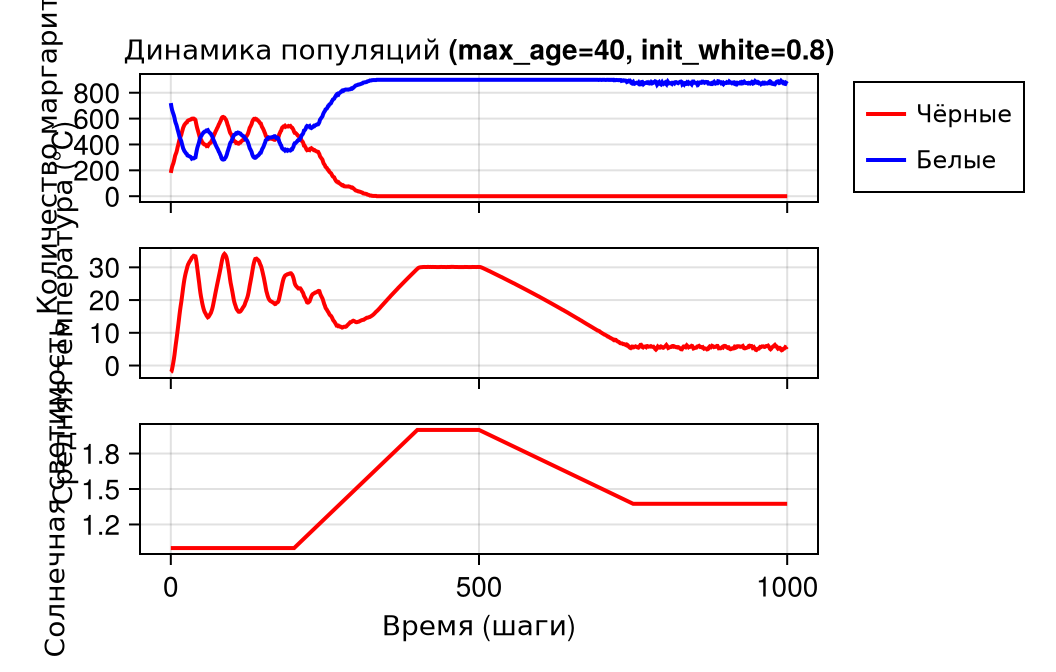
\includegraphics{simmod-lab03-report (Нджову Нелиа)_files/figure-pdf/cell-64-output-6.png}

\section{Итоги
эксперимента}\label{ux438ux442ux43eux433ux438-ux44dux43aux441ux43fux435ux440ux438ux43cux435ux43dux442ux430-1}

\begin{Shaded}
\begin{Highlighting}[]
\FunctionTok{println}\NormalTok{(}\StringTok{"ИТОГИ ПАРАМЕТРИЧЕСКОГО ИССЛЕДОВАНИЯ (СЦЕНАРИЙ :ramp)"}\NormalTok{)}
\FunctionTok{println}\NormalTok{(}\StringTok{"Всего выполнено экспериментов: "}\NormalTok{, }\FunctionTok{length}\NormalTok{(params\_list))}
\FunctionTok{println}\NormalTok{(}\StringTok{"Всего создано графиков: "}\NormalTok{, }\FunctionTok{length}\NormalTok{(params\_list))}
\FunctionTok{println}\NormalTok{(}\StringTok{"Графики сохранены в каталоге: "}\NormalTok{, }\FunctionTok{plotsdir}\NormalTok{())}
\end{Highlighting}
\end{Shaded}

\begin{verbatim}
ИТОГИ ПАРАМЕТРИЧЕСКОГО ИССЛЕДОВАНИЯ (СЦЕНАРИЙ :ramp)
Всего выполнено экспериментов: 4
Всего создано графиков: 4
Графики сохранены в каталоге: /home/nelianjovu/work/study/2026-1/2026-1==study--simulationmod/2026-1--study--simulationmod/labs/lab03/project/plots
\end{verbatim}

\chapter{Выводы}\label{ux432ux44bux432ux43eux434ux44b}

Выполнив эту лабораторную работу, я использовала агентную модель для
моделирования daisyworld.


\printbibliography


\end{document}
